\documentclass[sigconf]{acmart}

\usepackage{booktabs} % For formal tables

\usepackage{latexsym}
\usepackage{makecell}
\usepackage{epsfig}
\usepackage{algorithm, algpseudocode}
\usepackage{booktabs}
\usepackage{multirow}
\usepackage{color}
\usepackage{subfigure}
\usepackage{url}
\usepackage{mathrsfs}
\usepackage{amsmath}
\usepackage{bm}
%\usepackage[small]{caption}


\setlength{\abovecaptionskip}{5pt}
\setlength{\belowcaptionskip}{5pt}
\setlength{\textfloatsep}{3pt plus 2pt minus 2pt}


\newcommand\BibTeX{B{\sc ib}\TeX}
\newcommand{\secref}[1]{Section \ref{#1}}
\newcommand{\figref}[1]{Figure \ref{#1}}
\newcommand{\eqnref}[1]{Eq. (\ref{#1})}
\newcommand{\exref}[1]{Example \ref{#1}}
\newcommand{\algoref}[1]{Algorithm \ref{#1}}
\newcommand{\tabref}[1]{Table \ref{#1}}
\newcommand{\bi}[1]{\textbf{\textit{#1}}}
\newcommand{\KZ}[1]{\textcolor{red}{Kenny: #1}}
\newcommand{\XS}[1]{\textcolor{blue}{Xusheng: #1}}

% Copyright
\setcopyright{none}
%\setcopyright{acmcopyright}
%\setcopyright{acmlicensed}
%\setcopyright{rightsretained}
%\setcopyright{usgov}
%\setcopyright{usgovmixed}
%\setcopyright{cagov}
%\setcopyright{cagovmixed}


% DOI
\acmDOI{10.475/123_4}

% ISBN
\acmISBN{123-4567-24-567/08/06}

%Conference
\acmConference[KDD'19]{ACM SIGKDD Conference On Knowledge Discovery and Data Mining}{August 2019}{Anchorage, Alaska USA}
\acmYear{2019}
\copyrightyear{2019}


\acmArticle{4}
\acmPrice{15.00}

% These commands are optional
%\acmBooktitle{Transactions of the ACM Woodstock conference}


\begin{document}
\title{Inferring User Needs in E-commerce Recommendation}

\author{Xusheng Luo}
\affiliation{\institution{Alibaba Group}}
\email{lxs140564@alibaba-inc.com}

\author{Yonghua Yang}
\affiliation{\institution{Alibaba Group}}
\email{huazai.yyh@alibaba-inc.com}

\author{Keping Yang}
\affiliation{\institution{Alibaba Group}}
\email{shaoyao@taobao.com}

\author{Kenny Q. Zhu }
\affiliation{\institution{Shanghai Jiao Tong University}}
\email{kzhu@cs.sjtu.edu.cn}

\begin{abstract}
%Personalized recommender systems are becoming increasingly important to satisfy various shopping needs of consumers.
%They have been ubiquitous in a number of e-commerce platforms such as Alibaba and Amazon.
%\KZ{Inferring a concept behind user activities; explain recommendations.}
%Understanding latent user needs in their shopping behaviors is
%critical to industry recommender systems in e-commerce.
Recommendations made by modern e-commerce recommender systems are not driven
by user needs, and cannot explain the reason behind the decision.
%We believe, beneath the observable user behaviors such as clicks and 
%purchases, 
%\XS{Interpretability is one thing, another thing is novelty}
Representing implicit user needs explicitly as ``outdoor barbecue'' 
or ``keep warm for kids'' can further improve accuracy, novelty and interpretability
%offers great interpretability 
for recommender systems and ultimately leads to higher user satisfaction.
Backed by an e-commerce knowledge graph, 
%which is called \textbf{``E-commerce Concept Net''}, 
we propose a supervised learning algorithm to conceptualize user needs from 
their transaction history as ``concept'' nodes in the graph 
and then infer those concepts for each user
through a deep attentive model.
Offline experiments demonstrate the effectiveness and stability of our model,
and online industry strength tests show great advantages of such 
user needs understanding.
%Empowered by the e-commerce concept net,
%our solution might enlighten the next generation of e-commerce recommender systems.
\end{abstract}

%
% The code below should be generated by the tool at
% http://dl.acm.org/ccs.cfm
% Please copy and paste the code instead of the example below.
%



%\keywords{ACM proceedings, \LaTeX, text tagging}



\maketitle

%\IEEEraisesectionheading{
% %\IEEEraisesectionheading{
% %\IEEEraisesectionheading{
% \input{intro}
\section{Introduction}\label{sec:intro}
 %}
% \section{Introduction}\label{sec:intro}

% \begin{enumerate}
% \item Motivation: application scenarios (with 1-2 running examples);
% \item Characteristics of the data sources and their challenges;
% \item Briefly introduce previous approaches to extract information 
% from images including setting the document zone, and their limitations.
% \item General flow of our approach (may give a diagram here)
% \end{enumerate}
% scenary

Due to ever evolving hardware and software, many medical images
such as electro-cardio graphs (ECGs), X-ray or ultrasound images  
are directly printed and stored in hard copy formats. 
% \KZ{Insert 4 example images here.}
%Examples are shown in \figref{fig:medicalImages}. 
% These images often contain a mix of graphics and text, which
% include parameter settings of the hardware, test measurements or simple
% diagnosis. 
These images often contain a mix of graphics and text, which 
include technical settings of the hardware used, test measurements or simple diagnoses.
Recently, there has been a growing demand for digitizing such 
medical information from paper media sources, especially legacy ones, or patients who want to keep track of these documents by themselves digitally. 
Apart from scanning the graphics into a digital format, extracting 
the semi-structured textual information is also an important part of
building electronic medical records for patients. 

%\begin{figure}[!htb]
%\centering
%\subfloat[ECG]{
%\label{fig:medicalimage:ecg}
%\epsfig{file=figure/17_ori.eps, width=0.4\columnwidth}
%}
%% \hfill
%\subfloat[MRI]{
%	\label{fig:medicalimage:mrt}
%	\epsfig{file=figure/MRI.eps, width=0.4\columnwidth}
%}
%\\
%\subfloat[X-RAY]{
%\label{fig:medicalimage:xray}
%\epsfig{file=figure/X-RAY.eps, width=0.4\columnwidth}
%}
%%\hfill
%\subfloat[EEG]{
%\label{fig:medicalimage:eeg}
%\epsfig{file=figure/EEG.eps, width=0.4\columnwidth}
%}
%\caption{Examples of Medical Images}
%\label{fig:medicalImages}
%\end{figure}

Optical character recognition (OCR)  \cite{mori1992historical,smith2007overview} is 
a traditional technique used to turn images of printed text into machine encoded
text. It is well researched and performs well on plain text 
documents such as novels and reports, for a variety of languages. 
%For example, Tesseract, which is one of 
%the most popular open source multilingual recognizers, logs an error 
%rate of 3.72\% for English words and 3.77\% for simplified 
%Chinese characters\cite{smith2009adapting}. 
%Google Books \cite{googlebooks} and Gutenberg \cite{gutenberg} are
%projects which have scanned a large number of paper books into text for free and open
%access. These projects made exclusive use of OCR for this conversion and 
%achieved high accuracy \cite{vincent2007google} \cite{lebert2008project}. 
% 99\% for Gutenberg project \cite{lebert2008project}. 
% \KZ{Give the accuracy of google and gutenberg if available.}


\begin{figure}[th]
\centering
\epsfig{file=figure/17_b.eps, width=0.8\columnwidth}
\caption{An ECG image with text area (red circle) of interest.}
\label{fig:ecgexample2}
\end{figure}

For a semi-structured medical image, such as 
\figref{fig:ecgexample2}, we would like to extract the attribute-value 
pairs (e.g., {\em Vent. rate = 63 bpm}) and possibly other values such as
date ({\em 18-Nov-2010}) and time ({\em 9:13:02}) since those values endow us with lots of information about the patient. 
Existing OCR software cannot extract such structured information in a straightforward 
fashion, 
but instead it produces rather convoluted results from the whole image, 
similar to those in \figref{fig:ocrre}, which was produced by Tesseract, 
a popular multi-lingual recognizers. 
% \KZ{Maybe include the x-y coordinate info in the output as well?}  

\begin{figure}[th]
\centering
\scriptsize
\begin{verbatim}
<p class="ocr_par" title="box 263 33 444 119">
   <span class="ocr_l" title="box 264 33 336 45">
       <span class="ocrx_w" title="box 264 33 299 45">Vcnt.</span> 
       <span class="ocrx_w" title="box 308 34 336 45">rule</span> 
   </span>
   <span class='ocr_l'>
       <span class="ocrx_w" title="box 264 51 283 64">PR</span> 
       <span class="ocrx_w" title="box 291 51 346 64">Interval</span> 
       <span class="ocrx_w" title="box 389 52 411 64">140</span> 
       <span class="ocrx_w" title="box 420 55 439 64">ms</span> 
   </span>
   ...
   </span>
</p>
<p class="ocr_p" dir="ltr">
   <span class="ocr_l">
       <span class="ocrx_w" title="box 396 33 411 45">53</span> 
       <span class="ocrx_w" title="box 420 33 449 48">bpm</span> 
   </span>
</p>
\end{verbatim}
\caption{Snippet OCR results in XML, input to our framework.}
\label{fig:ocrre}
\end{figure}


%\input{xmlre1}

%However, OCR alone does not work well on semi-structured text and hence
%can't be directly used for information extraction from the aforementioned
%medical images. \KZ{Give the reason here, perhaps because OCR models are
%largely Markov based? So semi-structured data breaks the flow of text.}
%When a medical image is input to an ordinary OCR software, the spatial 
%information of the text components is often lost or mixed with noises
%and errors.
%%The reason is OCR converts the whole images into text data, in which 
%%useful information often mix with noises and errors. 
%In this paper, we would like to extract the attribute-value pairs
%and possibly other values from \figref{fig:ecgexample1} 
%and \figref{fig:ecgexample2}. 
%% or medical ultrasonography report. 
%Such images contain lots of non-textual information or noises.

% example & ref
%\begin{figure}[ht]
%\centering
%\epsfig{file=figure/46.eps, width=0.8\columnwidth}
%\caption{ECG Images From Printer1}
%\label{fig:ecgexample1}
%\end{figure}

% \begin{figure}[ht]
% \centering
% \subfloat[Printer1]{
% \label{fig:ecgexample:a}
% \epsfig{file=figure/46.eps, width=0.48\columnwidth}
% }
% \hfill
% \subfloat[Printer2]{
% \label{fig:ecgexample:b}
% \epsfig{file=figure/17.eps, width=0.48\columnwidth}
% }
% \caption{ECG images from two different printers}
% \label{fig:ecgexample}
% \end{figure}

Also, errors in the OCR text \cite{darwish2007error,taghva1996evaluation} will greatly affect the effectiveness 
of other related tasks. Much work has been done to improve the performance of the OCR\cite{kolak2003generative,cesarini1998informys}. However, there are still a number of significant challenges involved in extracting the information from medical images or OCR results in XML form. 

% First, medical images differ from pure text document in that them have 
% layout information. 
First, medical images differ from pure text documents in that 
they contain layout information.
Although most current OCR engines attempt to reproduce the physical 
layout of the text units, 
%(along with X-Y coordinates) and store them 
%in a special format such as XML 
% (\KZ{Better in the previous example})
such spatial
information is approximate and sometimes inaccurate, which is why neighboring
text blocks in \figref{fig:ecgexample2}, such as ``Vent. Rate'' and
``63 bpm'' were not automatically combined into the same XML block, but were 
rather far apart (shown in two different ``classes'') in \figref{fig:ocrre} made by OCR softwares. 
%Even for images produced by the same ECG printer, 
%the XML results can still be very different as 
The spatial layout is sensitive to many factors, such as accidental spots 
on the prints, color and contrast, or the angle of the camera. 
%In this case, solutions for other application domains, for example, the web, 
%are not well suited for information extraction from printed documents \cite{bartoli2014semisupervised}. With such inaccurate
%layout information produced by OCR,
%it is not easy to write a simple wrapper program to extract useful
%data from images, even if the images come from the same printer. 

%Writing a wrapper for each
%individual image would be tedious and counter-productive. Therefore,
%a mechanism that makes use of the spatial locality of the 
%text units in the image and 
%accommodates slight variations in the spatial layout would make the extraction
%more accurate and fault-tolerant.

%For example, \figref{fig:ocrre} is the simplified OCR results for the ECGs in 
%\figref{fig:ecgexample1} and \figref{fig:ecgexample2}. The results are in the XML format and have attritube named {\em class} 
%for layout information. Although these two images share similar format. 
%OCR engine generates different results in that it splits elements that 
%should be in the same line into two lines in the second example. 
%XML is sensitive to the layout results so it's hard to tolerate 
%all the layout results. 
%
% example check the term
% layout of ocr results can be restore, so why OCR engine don't restore the results 
% using the similar methods as we do?
% or the way we handle the layout problem is quite simple

% Delete for TIP
% Second, exiting OCR engines make heavy use of Markov properties such as n-grams
% since they primarily target the transformation of large body of text 
% \cite{kolak2003generative}. 
% % \KZ{Needs some refs here.}
% Unfortunately, the semi-structured texts in medical images are often 
% short and not even written in complete sentences, thus breaking Markov assumption. To make
% matters worse, medical images contain scientific language, which may be
% very different from the training corpora of these OCR engines.
% This explains why we see errors like ``Vcnt'' and ``rule'' 
% in \figref{fig:ocrre}. 
% %can't guarantee a perfect performance, which means 
% %there are errors and noises in the OCR results.
% %Many of them due to the fact that the data are no longer long, continous
% %sentences, thus breaking the Markov assumption made by many OCR algorithms. 
% %In \figref{fig:ocrresub:b}, ``Vent." is misrecognized as ``Vcnt.". 
% Without sufficient contextual information, OCR may also misrecognize a 
% digit as an alphabetic character, or as another similar digit. 
% Furthermore, the mix of text with images and formatting
% lines often confuses the OCR engine, which is more biased toward full
% text images.
% Exact pattern matching, as used in
% traditional information extraction, doesn't work with such noisy OCR output
% as it doesn't tolerate noises or errors in text. 
% %It's hard to autocorrect these errors 
% %because image quality is the most important affecting factor. 
% %The text we are processing can be full of no meaning words or 
% %strange numbers. 
% A fuzzy matching strategy is more desirable in this case. 
% % example, what are the traditional IEs

Second, there are many types of medical images, resulting from a variety of
medical tests. Different equipments for the same test can produce vastly 
different images. Writing individual extraction wrappers 
for the OCR outputs of all these formats is tedious and inefficient, 
and difficult for non-programmers.
%not to mention that there are significant programming barriers for 
%writing these wrappers, especially for the medical professionals who are the
%end users of these extraction results. 
%A more user-friendly approach enabling users to specify such extraction requirements would be preferred. 
%There are various kinds of medical images, such as electrocardiograph report, 
%medical ultrasonography report, etc. 
%However the basic measures for each type of medical test (e.g., ECG), 
%are very similar from machine to machine. Only the layouts are 
%different. 
% example medical images

Finally, most off-the-shelf OCR programs are pre-trained with specific 
recognition models, which may not be suitable for the extraction of 
%medical images.
%Furthermore, changes in imaging equipment technology over time may produce 
%different formats, layout, or terminology, rendering existing OCR models 
%obsolete. 
Re-training the models requires a large amount of labeled data, which may
not be available. 
%Incremental training as more labeled data arrives
%is currently not supported by any OCR product.    

%There have been some limited attempts to address some of the above challenges. 
%One solution is a plugin of an OCR program that allows the user to specify 
%target zones of interest in the image to be extracted. The zones specified for
%one image can be applied to images with slight variations by adjusting against
%a fixed reference point that is supposed to exist in all these images.
%% \KZ{I think the problem is not so much with the zones, because we also
%% have zones, but rather with the reference point.}
%% \JY{}
%% example products
%% http://www.square-9.com/automated-data-extraction-optical-character-recognition
%The problem with this solution is its high reliance on the OCR zones  
%established by the user. The performance of the results is affected by the 
%accuracy of the zones. If the zones are too big, the results will be full of 
%noise. If the zones are too small, results will miss something. 
%
%Another solution involves using the page layout analysis technique. The page layout 
%analysis technique is used to determine where the text 
%resides on a page \cite{o1993document}, 
%% \KZ{This page layout analysis approach is not clearly described. I don't understand after reading this paragraph.}
%% By using page layout analysis technique, the hierarchy of physical components 
%% can be generated and to match with the hierarchy of logical components, which 
%% is predefined. 
%this includes identifying and categorizing the 
%regions of interest in the scanned image of a text document. 
%Typically, the first step is to segment text zones from 
%non-textual zones and arrange them in their original order. 
%Then in order to analyze the logical roles of the text zones 
%(titles, captions, footnotes, etc.), logical layout analysis 
%is used for labeling the semantics of the text zones.
%Generally, page layout analysis is used for documents. The problem with applying 
%such a technique on medical images is that it creates so much noises 
%that performance is ultimately affected. 
%For medical imaging reports like ECG, useful information is often 
%found in the small components of the image, while most of the images are 
%read as noises. 
% check paper and more description, weakness, ref

%In this paper, 
%we propose a spatial data description language, which borrows its syntax from
%PADS \cite{fisher+:pads}, an ad hoc data processing language, 
%for describing semi-structured data in medical images. 
%% ref
%We call this language OCR description language, or ODL. 
%ODL is designed for extracting and parsing semi-structured text data 
%from images. We believe that  information extraction from those data in ODL form may be much easier than extracting information from rough data or data in XML form, which means that our preprocessing part proves to be necessary.
%%An example ODL description for the image in 
%%\figref{fig:ecgexample2} is shown in 
%%\figref{fig:description}. \KZ{Make this description two column, and give
%%some brief explanation of this description here.} 
%%The parsing result of this description is shown
%%in \figref{fig:parsing result}. \KZ{Give some explanation of the results,
%%otherwise don't show the result here. E.g., you need to explain what F, E, etc.
%%mean. You want to say that even though rate has been recognized as rule,
%%the bpm value was still extracted (but still wrong!).}
%% \KZ{I removed the preprocessing part, cos it's not important. Talk about it in
%% discussion sec.}
%%The our approach starts by preprocessing the images for text results.
%To use this framework, the user first describes the components in the image
%that he or she is interested in extracting. This includes constant strings
%and variables of different data types.   
%ODL allows the user to specify the approximate spatial layout and constraints on
%the data, e.g., integers within 
%a certain range, real numbers with certain decimal points, etc. 
%%This information is then as the key component in our fuzzy matching strategy. 
%The system then automatically generates a parser for these medical images.
%This parser uses the output XML from OCR with spatial information as an input, 
%and outputs a data structure with values extracted for each variables
%in the description, unless there is an unrecoverable error during the parsing process.
%In addition, approximate layout information and constraints are used in parsing process 
%to tolerate noises and small format variations in the input images. 
%%Specifically, this method could be called fuzzy matching, meaning that more candidates could be saved after the parsing process.  It's obvious that we may have a higher probability to obtain the accurate result if more candidates are kept so that fuzzy match should be used properly in our system.
%%An autogenerated parser based on the ODL description can release us from 
%%repetitive work. In this way, we turn the task of writing complex parsers 
%%into describing information on images.
%
%
%When users process many images of the same format, the system 
%automatically discovers parsing errors given the current model and 
%prompts the user to manually correct some of the frequent and prominent
%errors, which effectively serves as an online labeling function. 
%These incrementally labeled data are then used to update the parsing model. 


%It should be emphasized that the incremental learning model is very important in our whole system. Incremental learning is a machine learning paradigm where the learning process takes place whenever we have new examples or data added to our baisc data set, leading to a most striking difference between incremental learning and traditional machine learning: it does not assume the availability of a sufficient training set before the learning process. What incremental learning in our system is really impressive: it does not require a relatively good and stable training set at first time. In fact, it could improve the parsing result with even relatively rough training sets at first by absorbing new data or corrective information as time passes in dynamic systems. Besides, the process would be very effective when there are some new images coming in since training process would not learn from scratch, which might waste time and computation resource.

%At last, we propose an incrementally human correction framwork which can 
%make the best use of human correction to handle the misrecognition problem. 
% Base on our experiments on about 500 real life ECG images, 
% our approach achieves p1 and p2 after p3 times human correction. 
% experimental results

% \begin{figure}[h]
% \begin{lstlisting}
% Oenum str_month_t{
% 	"Jan", "Feb", "Mar", "Apr",
% 	"May", "Jun", "Jul", "Aug",
% 	"Sept", "Oct", "Nov", "Dec"
% };

% Ounion month_t{
% 	Oint(1,12)	num;
% 	str_month_t	str;
% };

% Ostruct time_t{
% 	Oint(1,31)	day;
% 	"-";
% 	month_t	month;
% 	"-";
% 	Oint	year;
% };

% Ostruct triple_t{
% 	"Vent.";
% 	hskip(\s)	skip1;
% 	"rate";
% 	Oint x;
% 	"bpm";
% 	vskip(\n)	skip2;
% };

% Oscource Ostruct entry_t{
% 	time_t(<-,-,-,0.3l>) t;
% 	triple_t(<0.1w,-,0.5w,->) d;
% };
% \end{lstlisting}
% \caption{Description}\label{fig:description}
% \end{figure}


In order to solve above problems, We design a system which makes three main contributions:
\begin{enumerate}
\item Based on some previous work on data description language \cite{lamport1986document,taft1999post,fisher+:pads},we design a new declarative spatial data description language called \textit{OCR description language}, or ODL,
which allows users to specify spatial and data constraints in medical 
images(\secref{sec:syntax});
\item We propose a noise-tolerant parser which takes OCR results
the ODL description as input and outputs a data structure with values 
extracted for each variables in the description (\secref{sec:semantics});
\item We propose an incremental manual correction 
framework\cite{von2008recaptcha,zhu2012learnpads++}, which 
takes advantage of user corrections  and improves the productivity
significantly (\secref{sec:correction}).
%To be more specific, the framework improves the traditional machine learning methods by using a incremental learning process to avoid starting from scratch when we are trying to apply human corrections in the system. That means the framework would be more effective than most corrective systems.
\end{enumerate}


\section{Introduction}\label{sec:intro}
 %}
% \section{Introduction}\label{sec:intro}

% \begin{enumerate}
% \item Motivation: application scenarios (with 1-2 running examples);
% \item Characteristics of the data sources and their challenges;
% \item Briefly introduce previous approaches to extract information 
% from images including setting the document zone, and their limitations.
% \item General flow of our approach (may give a diagram here)
% \end{enumerate}
% scenary

Due to ever evolving hardware and software, many medical images
such as electro-cardio graphs (ECGs), X-ray or ultrasound images  
are directly printed and stored in hard copy formats. 
% \KZ{Insert 4 example images here.}
%Examples are shown in \figref{fig:medicalImages}. 
% These images often contain a mix of graphics and text, which
% include parameter settings of the hardware, test measurements or simple
% diagnosis. 
These images often contain a mix of graphics and text, which 
include technical settings of the hardware used, test measurements or simple diagnoses.
Recently, there has been a growing demand for digitizing such 
medical information from paper media sources, especially legacy ones, or patients who want to keep track of these documents by themselves digitally. 
Apart from scanning the graphics into a digital format, extracting 
the semi-structured textual information is also an important part of
building electronic medical records for patients. 

%\begin{figure}[!htb]
%\centering
%\subfloat[ECG]{
%\label{fig:medicalimage:ecg}
%\epsfig{file=figure/17_ori.eps, width=0.4\columnwidth}
%}
%% \hfill
%\subfloat[MRI]{
%	\label{fig:medicalimage:mrt}
%	\epsfig{file=figure/MRI.eps, width=0.4\columnwidth}
%}
%\\
%\subfloat[X-RAY]{
%\label{fig:medicalimage:xray}
%\epsfig{file=figure/X-RAY.eps, width=0.4\columnwidth}
%}
%%\hfill
%\subfloat[EEG]{
%\label{fig:medicalimage:eeg}
%\epsfig{file=figure/EEG.eps, width=0.4\columnwidth}
%}
%\caption{Examples of Medical Images}
%\label{fig:medicalImages}
%\end{figure}

Optical character recognition (OCR)  \cite{mori1992historical,smith2007overview} is 
a traditional technique used to turn images of printed text into machine encoded
text. It is well researched and performs well on plain text 
documents such as novels and reports, for a variety of languages. 
%For example, Tesseract, which is one of 
%the most popular open source multilingual recognizers, logs an error 
%rate of 3.72\% for English words and 3.77\% for simplified 
%Chinese characters\cite{smith2009adapting}. 
%Google Books \cite{googlebooks} and Gutenberg \cite{gutenberg} are
%projects which have scanned a large number of paper books into text for free and open
%access. These projects made exclusive use of OCR for this conversion and 
%achieved high accuracy \cite{vincent2007google} \cite{lebert2008project}. 
% 99\% for Gutenberg project \cite{lebert2008project}. 
% \KZ{Give the accuracy of google and gutenberg if available.}


\begin{figure}[th]
\centering
\epsfig{file=figure/17_b.eps, width=0.8\columnwidth}
\caption{An ECG image with text area (red circle) of interest.}
\label{fig:ecgexample2}
\end{figure}

For a semi-structured medical image, such as 
\figref{fig:ecgexample2}, we would like to extract the attribute-value 
pairs (e.g., {\em Vent. rate = 63 bpm}) and possibly other values such as
date ({\em 18-Nov-2010}) and time ({\em 9:13:02}) since those values endow us with lots of information about the patient. 
Existing OCR software cannot extract such structured information in a straightforward 
fashion, 
but instead it produces rather convoluted results from the whole image, 
similar to those in \figref{fig:ocrre}, which was produced by Tesseract, 
a popular multi-lingual recognizers. 
% \KZ{Maybe include the x-y coordinate info in the output as well?}  

\begin{figure}[th]
\centering
\scriptsize
\begin{verbatim}
<p class="ocr_par" title="box 263 33 444 119">
   <span class="ocr_l" title="box 264 33 336 45">
       <span class="ocrx_w" title="box 264 33 299 45">Vcnt.</span> 
       <span class="ocrx_w" title="box 308 34 336 45">rule</span> 
   </span>
   <span class='ocr_l'>
       <span class="ocrx_w" title="box 264 51 283 64">PR</span> 
       <span class="ocrx_w" title="box 291 51 346 64">Interval</span> 
       <span class="ocrx_w" title="box 389 52 411 64">140</span> 
       <span class="ocrx_w" title="box 420 55 439 64">ms</span> 
   </span>
   ...
   </span>
</p>
<p class="ocr_p" dir="ltr">
   <span class="ocr_l">
       <span class="ocrx_w" title="box 396 33 411 45">53</span> 
       <span class="ocrx_w" title="box 420 33 449 48">bpm</span> 
   </span>
</p>
\end{verbatim}
\caption{Snippet OCR results in XML, input to our framework.}
\label{fig:ocrre}
\end{figure}


%% \begin{figure}[ht]
% \centering
% \subfigure[]{
% \label{fig:subfig:a}
% \begin{minipage}[b]{0.2\textwidth}
%\newsavebox{\firstlisting}
%\begin{lrbox}{\firstlisting}% Store first listing
%\begin{lstlisting}
%<p class='ocr_par' dir='ltr'>
%   <span class='ocr_line' id='line_2'>
%       <span class='ocrx_word' id='word_6'>Vent.</span>
%       <span class='ocrx_word' id='word_7'>rate</span>
%       <span class='ocrx_word' id='word_8'>65</span>
%       <span class='ocrx_word' id='word_9'>bpm</span>
%   </span>
%   <span class='ocr_line' id='line_3'>
%       <span class='ocrx_word' id='word_14'>PR</span>
%       <span class='ocrx_word' id='word_15'>interval</span>
%       <span class='ocrx_word' id='word_16'>162</span>
%       <span class='ocrx_word' id='word_17'>ms</span>
%   </span>
%    ...
%</p>
%\end{lstlisting}
%\end{lrbox}
% \end{minipage}
% }
% \hspace[1in]
% \subfigure[]{
% % \label{fig:subfig:b}
% % \begin{minipage}[b]{0.2\textwidth}
\newsavebox{\secondlisting}
\begin{lrbox}{\secondlisting}
% \tiny
\begin{lstlisting}[basicstyle=\tiny,]
<p class="ocr_par" title="box 263 33 444 119">
   <span class="ocr_l" title="box 264 33 336 45">
       <span class="ocrx_w" title="box 264 33 299 45">Vcnt.</span>
       <span class="ocrx_w" title="box 308 34 336 45">rule</span>
   </span>
   <span class='ocr_l'>
       <span class="ocrx_w" title="box 264 51 283 64">PR</span>
       <span class="ocrx_w" title="box 291 51 346 64">Interval</span>
       <span class="ocrx_w" title="box 389 52 411 64">140</span>
       <span class="ocrx_w" title="box 420 55 439 64">ms</span>
   </span>
   ...
   </span>
</p>
<p class="ocr_p" dir="ltr">
   <span class="ocr_l">
       <span class="ocrx_w" title="box 396 33 411 45">53</span>
       <span class="ocrx_w" title="box 420 33 449 48">bpm</span>
   </span>
</p>
\end{lstlisting}
\end{lrbox}
% % \end{minipage}
% }

% \KZ{\figref{fig:ocrre} is output from what software? Tesseract?}
\begin{figure*}[th]
%\subfloat[Image From Printer1]{
%\label{fig:ocrresub:a}
%\scalebox{0.8}{\usebox{\firstlisting}}}
%\hfill
%\subfloat[Image From Printer2]{
\scalebox{1.6}{\usebox{\secondlisting}}
% \label{fig:ocrre}
\caption{A fragment of raw OCR results for ECG with layout information.}
%\caption{Simplified OCR Results in XML for an ECG with Layout Information}
%\label{fig:ocrresub:b}
\label{fig:running-xml}
\end{figure*}

% \lipsum[2]


%However, OCR alone does not work well on semi-structured text and hence
%can't be directly used for information extraction from the aforementioned
%medical images. \KZ{Give the reason here, perhaps because OCR models are
%largely Markov based? So semi-structured data breaks the flow of text.}
%When a medical image is input to an ordinary OCR software, the spatial 
%information of the text components is often lost or mixed with noises
%and errors.
%%The reason is OCR converts the whole images into text data, in which 
%%useful information often mix with noises and errors. 
%In this paper, we would like to extract the attribute-value pairs
%and possibly other values from \figref{fig:ecgexample1} 
%and \figref{fig:ecgexample2}. 
%% or medical ultrasonography report. 
%Such images contain lots of non-textual information or noises.

% example & ref
%\begin{figure}[ht]
%\centering
%\epsfig{file=figure/46.eps, width=0.8\columnwidth}
%\caption{ECG Images From Printer1}
%\label{fig:ecgexample1}
%\end{figure}

% \begin{figure}[ht]
% \centering
% \subfloat[Printer1]{
% \label{fig:ecgexample:a}
% \epsfig{file=figure/46.eps, width=0.48\columnwidth}
% }
% \hfill
% \subfloat[Printer2]{
% \label{fig:ecgexample:b}
% \epsfig{file=figure/17.eps, width=0.48\columnwidth}
% }
% \caption{ECG images from two different printers}
% \label{fig:ecgexample}
% \end{figure}

Also, errors in the OCR text \cite{darwish2007error,taghva1996evaluation} will greatly affect the effectiveness 
of other related tasks. Much work has been done to improve the performance of the OCR\cite{kolak2003generative,cesarini1998informys}. However, there are still a number of significant challenges involved in extracting the information from medical images or OCR results in XML form. 

% First, medical images differ from pure text document in that them have 
% layout information. 
First, medical images differ from pure text documents in that 
they contain layout information.
Although most current OCR engines attempt to reproduce the physical 
layout of the text units, 
%(along with X-Y coordinates) and store them 
%in a special format such as XML 
% (\KZ{Better in the previous example})
such spatial
information is approximate and sometimes inaccurate, which is why neighboring
text blocks in \figref{fig:ecgexample2}, such as ``Vent. Rate'' and
``63 bpm'' were not automatically combined into the same XML block, but were 
rather far apart (shown in two different ``classes'') in \figref{fig:ocrre} made by OCR softwares. 
%Even for images produced by the same ECG printer, 
%the XML results can still be very different as 
The spatial layout is sensitive to many factors, such as accidental spots 
on the prints, color and contrast, or the angle of the camera. 
%In this case, solutions for other application domains, for example, the web, 
%are not well suited for information extraction from printed documents \cite{bartoli2014semisupervised}. With such inaccurate
%layout information produced by OCR,
%it is not easy to write a simple wrapper program to extract useful
%data from images, even if the images come from the same printer. 

%Writing a wrapper for each
%individual image would be tedious and counter-productive. Therefore,
%a mechanism that makes use of the spatial locality of the 
%text units in the image and 
%accommodates slight variations in the spatial layout would make the extraction
%more accurate and fault-tolerant.

%For example, \figref{fig:ocrre} is the simplified OCR results for the ECGs in 
%\figref{fig:ecgexample1} and \figref{fig:ecgexample2}. The results are in the XML format and have attritube named {\em class} 
%for layout information. Although these two images share similar format. 
%OCR engine generates different results in that it splits elements that 
%should be in the same line into two lines in the second example. 
%XML is sensitive to the layout results so it's hard to tolerate 
%all the layout results. 
%
% example check the term
% layout of ocr results can be restore, so why OCR engine don't restore the results 
% using the similar methods as we do?
% or the way we handle the layout problem is quite simple

% Delete for TIP
% Second, exiting OCR engines make heavy use of Markov properties such as n-grams
% since they primarily target the transformation of large body of text 
% \cite{kolak2003generative}. 
% % \KZ{Needs some refs here.}
% Unfortunately, the semi-structured texts in medical images are often 
% short and not even written in complete sentences, thus breaking Markov assumption. To make
% matters worse, medical images contain scientific language, which may be
% very different from the training corpora of these OCR engines.
% This explains why we see errors like ``Vcnt'' and ``rule'' 
% in \figref{fig:ocrre}. 
% %can't guarantee a perfect performance, which means 
% %there are errors and noises in the OCR results.
% %Many of them due to the fact that the data are no longer long, continous
% %sentences, thus breaking the Markov assumption made by many OCR algorithms. 
% %In \figref{fig:ocrresub:b}, ``Vent." is misrecognized as ``Vcnt.". 
% Without sufficient contextual information, OCR may also misrecognize a 
% digit as an alphabetic character, or as another similar digit. 
% Furthermore, the mix of text with images and formatting
% lines often confuses the OCR engine, which is more biased toward full
% text images.
% Exact pattern matching, as used in
% traditional information extraction, doesn't work with such noisy OCR output
% as it doesn't tolerate noises or errors in text. 
% %It's hard to autocorrect these errors 
% %because image quality is the most important affecting factor. 
% %The text we are processing can be full of no meaning words or 
% %strange numbers. 
% A fuzzy matching strategy is more desirable in this case. 
% % example, what are the traditional IEs

Second, there are many types of medical images, resulting from a variety of
medical tests. Different equipments for the same test can produce vastly 
different images. Writing individual extraction wrappers 
for the OCR outputs of all these formats is tedious and inefficient, 
and difficult for non-programmers.
%not to mention that there are significant programming barriers for 
%writing these wrappers, especially for the medical professionals who are the
%end users of these extraction results. 
%A more user-friendly approach enabling users to specify such extraction requirements would be preferred. 
%There are various kinds of medical images, such as electrocardiograph report, 
%medical ultrasonography report, etc. 
%However the basic measures for each type of medical test (e.g., ECG), 
%are very similar from machine to machine. Only the layouts are 
%different. 
% example medical images

Finally, most off-the-shelf OCR programs are pre-trained with specific 
recognition models, which may not be suitable for the extraction of 
%medical images.
%Furthermore, changes in imaging equipment technology over time may produce 
%different formats, layout, or terminology, rendering existing OCR models 
%obsolete. 
Re-training the models requires a large amount of labeled data, which may
not be available. 
%Incremental training as more labeled data arrives
%is currently not supported by any OCR product.    

%There have been some limited attempts to address some of the above challenges. 
%One solution is a plugin of an OCR program that allows the user to specify 
%target zones of interest in the image to be extracted. The zones specified for
%one image can be applied to images with slight variations by adjusting against
%a fixed reference point that is supposed to exist in all these images.
%% \KZ{I think the problem is not so much with the zones, because we also
%% have zones, but rather with the reference point.}
%% \JY{}
%% example products
%% http://www.square-9.com/automated-data-extraction-optical-character-recognition
%The problem with this solution is its high reliance on the OCR zones  
%established by the user. The performance of the results is affected by the 
%accuracy of the zones. If the zones are too big, the results will be full of 
%noise. If the zones are too small, results will miss something. 
%
%Another solution involves using the page layout analysis technique. The page layout 
%analysis technique is used to determine where the text 
%resides on a page \cite{o1993document}, 
%% \KZ{This page layout analysis approach is not clearly described. I don't understand after reading this paragraph.}
%% By using page layout analysis technique, the hierarchy of physical components 
%% can be generated and to match with the hierarchy of logical components, which 
%% is predefined. 
%this includes identifying and categorizing the 
%regions of interest in the scanned image of a text document. 
%Typically, the first step is to segment text zones from 
%non-textual zones and arrange them in their original order. 
%Then in order to analyze the logical roles of the text zones 
%(titles, captions, footnotes, etc.), logical layout analysis 
%is used for labeling the semantics of the text zones.
%Generally, page layout analysis is used for documents. The problem with applying 
%such a technique on medical images is that it creates so much noises 
%that performance is ultimately affected. 
%For medical imaging reports like ECG, useful information is often 
%found in the small components of the image, while most of the images are 
%read as noises. 
% check paper and more description, weakness, ref

%In this paper, 
%we propose a spatial data description language, which borrows its syntax from
%PADS \cite{fisher+:pads}, an ad hoc data processing language, 
%for describing semi-structured data in medical images. 
%% ref
%We call this language OCR description language, or ODL. 
%ODL is designed for extracting and parsing semi-structured text data 
%from images. We believe that  information extraction from those data in ODL form may be much easier than extracting information from rough data or data in XML form, which means that our preprocessing part proves to be necessary.
%%An example ODL description for the image in 
%%\figref{fig:ecgexample2} is shown in 
%%\figref{fig:description}. \KZ{Make this description two column, and give
%%some brief explanation of this description here.} 
%%The parsing result of this description is shown
%%in \figref{fig:parsing result}. \KZ{Give some explanation of the results,
%%otherwise don't show the result here. E.g., you need to explain what F, E, etc.
%%mean. You want to say that even though rate has been recognized as rule,
%%the bpm value was still extracted (but still wrong!).}
%% \KZ{I removed the preprocessing part, cos it's not important. Talk about it in
%% discussion sec.}
%%The our approach starts by preprocessing the images for text results.
%To use this framework, the user first describes the components in the image
%that he or she is interested in extracting. This includes constant strings
%and variables of different data types.   
%ODL allows the user to specify the approximate spatial layout and constraints on
%the data, e.g., integers within 
%a certain range, real numbers with certain decimal points, etc. 
%%This information is then as the key component in our fuzzy matching strategy. 
%The system then automatically generates a parser for these medical images.
%This parser uses the output XML from OCR with spatial information as an input, 
%and outputs a data structure with values extracted for each variables
%in the description, unless there is an unrecoverable error during the parsing process.
%In addition, approximate layout information and constraints are used in parsing process 
%to tolerate noises and small format variations in the input images. 
%%Specifically, this method could be called fuzzy matching, meaning that more candidates could be saved after the parsing process.  It's obvious that we may have a higher probability to obtain the accurate result if more candidates are kept so that fuzzy match should be used properly in our system.
%%An autogenerated parser based on the ODL description can release us from 
%%repetitive work. In this way, we turn the task of writing complex parsers 
%%into describing information on images.
%
%
%When users process many images of the same format, the system 
%automatically discovers parsing errors given the current model and 
%prompts the user to manually correct some of the frequent and prominent
%errors, which effectively serves as an online labeling function. 
%These incrementally labeled data are then used to update the parsing model. 


%It should be emphasized that the incremental learning model is very important in our whole system. Incremental learning is a machine learning paradigm where the learning process takes place whenever we have new examples or data added to our baisc data set, leading to a most striking difference between incremental learning and traditional machine learning: it does not assume the availability of a sufficient training set before the learning process. What incremental learning in our system is really impressive: it does not require a relatively good and stable training set at first time. In fact, it could improve the parsing result with even relatively rough training sets at first by absorbing new data or corrective information as time passes in dynamic systems. Besides, the process would be very effective when there are some new images coming in since training process would not learn from scratch, which might waste time and computation resource.

%At last, we propose an incrementally human correction framwork which can 
%make the best use of human correction to handle the misrecognition problem. 
% Base on our experiments on about 500 real life ECG images, 
% our approach achieves p1 and p2 after p3 times human correction. 
% experimental results

% \begin{figure}[h]
% \begin{lstlisting}
% Oenum str_month_t{
% 	"Jan", "Feb", "Mar", "Apr",
% 	"May", "Jun", "Jul", "Aug",
% 	"Sept", "Oct", "Nov", "Dec"
% };

% Ounion month_t{
% 	Oint(1,12)	num;
% 	str_month_t	str;
% };

% Ostruct time_t{
% 	Oint(1,31)	day;
% 	"-";
% 	month_t	month;
% 	"-";
% 	Oint	year;
% };

% Ostruct triple_t{
% 	"Vent.";
% 	hskip(\s)	skip1;
% 	"rate";
% 	Oint x;
% 	"bpm";
% 	vskip(\n)	skip2;
% };

% Oscource Ostruct entry_t{
% 	time_t(<-,-,-,0.3l>) t;
% 	triple_t(<0.1w,-,0.5w,->) d;
% };
% \end{lstlisting}
% \caption{Description}\label{fig:description}
% \end{figure}


In order to solve above problems, We design a system which makes three main contributions:
\begin{enumerate}
\item Based on some previous work on data description language \cite{lamport1986document,taft1999post,fisher+:pads},we design a new declarative spatial data description language called \textit{OCR description language}, or ODL,
which allows users to specify spatial and data constraints in medical 
images(\secref{sec:syntax});
\item We propose a noise-tolerant parser which takes OCR results
the ODL description as input and outputs a data structure with values 
extracted for each variables in the description (\secref{sec:semantics});
\item We propose an incremental manual correction 
framework\cite{von2008recaptcha,zhu2012learnpads++}, which 
takes advantage of user corrections  and improves the productivity
significantly (\secref{sec:correction}).
%To be more specific, the framework improves the traditional machine learning methods by using a incremental learning process to avoid starting from scratch when we are trying to apply human corrections in the system. That means the framework would be more effective than most corrective systems.
\end{enumerate}


\section{Introduction}\label{sec:intro}
 %}
% \section{Introduction}\label{sec:intro}

% \begin{enumerate}
% \item Motivation: application scenarios (with 1-2 running examples);
% \item Characteristics of the data sources and their challenges;
% \item Briefly introduce previous approaches to extract information 
% from images including setting the document zone, and their limitations.
% \item General flow of our approach (may give a diagram here)
% \end{enumerate}
% scenary

Due to ever evolving hardware and software, many medical images
such as electro-cardio graphs (ECGs), X-ray or ultrasound images  
are directly printed and stored in hard copy formats. 
% \KZ{Insert 4 example images here.}
%Examples are shown in \figref{fig:medicalImages}. 
% These images often contain a mix of graphics and text, which
% include parameter settings of the hardware, test measurements or simple
% diagnosis. 
These images often contain a mix of graphics and text, which 
include technical settings of the hardware used, test measurements or simple diagnoses.
Recently, there has been a growing demand for digitizing such 
medical information from paper media sources, especially legacy ones, or patients who want to keep track of these documents by themselves digitally. 
Apart from scanning the graphics into a digital format, extracting 
the semi-structured textual information is also an important part of
building electronic medical records for patients. 

%\begin{figure}[!htb]
%\centering
%\subfloat[ECG]{
%\label{fig:medicalimage:ecg}
%\epsfig{file=figure/17_ori.eps, width=0.4\columnwidth}
%}
%% \hfill
%\subfloat[MRI]{
%	\label{fig:medicalimage:mrt}
%	\epsfig{file=figure/MRI.eps, width=0.4\columnwidth}
%}
%\\
%\subfloat[X-RAY]{
%\label{fig:medicalimage:xray}
%\epsfig{file=figure/X-RAY.eps, width=0.4\columnwidth}
%}
%%\hfill
%\subfloat[EEG]{
%\label{fig:medicalimage:eeg}
%\epsfig{file=figure/EEG.eps, width=0.4\columnwidth}
%}
%\caption{Examples of Medical Images}
%\label{fig:medicalImages}
%\end{figure}

Optical character recognition (OCR)  \cite{mori1992historical,smith2007overview} is 
a traditional technique used to turn images of printed text into machine encoded
text. It is well researched and performs well on plain text 
documents such as novels and reports, for a variety of languages. 
%For example, Tesseract, which is one of 
%the most popular open source multilingual recognizers, logs an error 
%rate of 3.72\% for English words and 3.77\% for simplified 
%Chinese characters\cite{smith2009adapting}. 
%Google Books \cite{googlebooks} and Gutenberg \cite{gutenberg} are
%projects which have scanned a large number of paper books into text for free and open
%access. These projects made exclusive use of OCR for this conversion and 
%achieved high accuracy \cite{vincent2007google} \cite{lebert2008project}. 
% 99\% for Gutenberg project \cite{lebert2008project}. 
% \KZ{Give the accuracy of google and gutenberg if available.}


\begin{figure}[th]
\centering
\epsfig{file=figure/17_b.eps, width=0.8\columnwidth}
\caption{An ECG image with text area (red circle) of interest.}
\label{fig:ecgexample2}
\end{figure}

For a semi-structured medical image, such as 
\figref{fig:ecgexample2}, we would like to extract the attribute-value 
pairs (e.g., {\em Vent. rate = 63 bpm}) and possibly other values such as
date ({\em 18-Nov-2010}) and time ({\em 9:13:02}) since those values endow us with lots of information about the patient. 
Existing OCR software cannot extract such structured information in a straightforward 
fashion, 
but instead it produces rather convoluted results from the whole image, 
similar to those in \figref{fig:ocrre}, which was produced by Tesseract, 
a popular multi-lingual recognizers. 
% \KZ{Maybe include the x-y coordinate info in the output as well?}  

\begin{figure}[th]
\centering
\scriptsize
\begin{verbatim}
<p class="ocr_par" title="box 263 33 444 119">
   <span class="ocr_l" title="box 264 33 336 45">
       <span class="ocrx_w" title="box 264 33 299 45">Vcnt.</span> 
       <span class="ocrx_w" title="box 308 34 336 45">rule</span> 
   </span>
   <span class='ocr_l'>
       <span class="ocrx_w" title="box 264 51 283 64">PR</span> 
       <span class="ocrx_w" title="box 291 51 346 64">Interval</span> 
       <span class="ocrx_w" title="box 389 52 411 64">140</span> 
       <span class="ocrx_w" title="box 420 55 439 64">ms</span> 
   </span>
   ...
   </span>
</p>
<p class="ocr_p" dir="ltr">
   <span class="ocr_l">
       <span class="ocrx_w" title="box 396 33 411 45">53</span> 
       <span class="ocrx_w" title="box 420 33 449 48">bpm</span> 
   </span>
</p>
\end{verbatim}
\caption{Snippet OCR results in XML, input to our framework.}
\label{fig:ocrre}
\end{figure}


%% \begin{figure}[ht]
% \centering
% \subfigure[]{
% \label{fig:subfig:a}
% \begin{minipage}[b]{0.2\textwidth}
%\newsavebox{\firstlisting}
%\begin{lrbox}{\firstlisting}% Store first listing
%\begin{lstlisting}
%<p class='ocr_par' dir='ltr'>
%   <span class='ocr_line' id='line_2'>
%       <span class='ocrx_word' id='word_6'>Vent.</span>
%       <span class='ocrx_word' id='word_7'>rate</span>
%       <span class='ocrx_word' id='word_8'>65</span>
%       <span class='ocrx_word' id='word_9'>bpm</span>
%   </span>
%   <span class='ocr_line' id='line_3'>
%       <span class='ocrx_word' id='word_14'>PR</span>
%       <span class='ocrx_word' id='word_15'>interval</span>
%       <span class='ocrx_word' id='word_16'>162</span>
%       <span class='ocrx_word' id='word_17'>ms</span>
%   </span>
%    ...
%</p>
%\end{lstlisting}
%\end{lrbox}
% \end{minipage}
% }
% \hspace[1in]
% \subfigure[]{
% % \label{fig:subfig:b}
% % \begin{minipage}[b]{0.2\textwidth}
\newsavebox{\secondlisting}
\begin{lrbox}{\secondlisting}
% \tiny
\begin{lstlisting}[basicstyle=\tiny,]
<p class="ocr_par" title="box 263 33 444 119">
   <span class="ocr_l" title="box 264 33 336 45">
       <span class="ocrx_w" title="box 264 33 299 45">Vcnt.</span>
       <span class="ocrx_w" title="box 308 34 336 45">rule</span>
   </span>
   <span class='ocr_l'>
       <span class="ocrx_w" title="box 264 51 283 64">PR</span>
       <span class="ocrx_w" title="box 291 51 346 64">Interval</span>
       <span class="ocrx_w" title="box 389 52 411 64">140</span>
       <span class="ocrx_w" title="box 420 55 439 64">ms</span>
   </span>
   ...
   </span>
</p>
<p class="ocr_p" dir="ltr">
   <span class="ocr_l">
       <span class="ocrx_w" title="box 396 33 411 45">53</span>
       <span class="ocrx_w" title="box 420 33 449 48">bpm</span>
   </span>
</p>
\end{lstlisting}
\end{lrbox}
% % \end{minipage}
% }

% \KZ{\figref{fig:ocrre} is output from what software? Tesseract?}
\begin{figure*}[th]
%\subfloat[Image From Printer1]{
%\label{fig:ocrresub:a}
%\scalebox{0.8}{\usebox{\firstlisting}}}
%\hfill
%\subfloat[Image From Printer2]{
\scalebox{1.6}{\usebox{\secondlisting}}
% \label{fig:ocrre}
\caption{A fragment of raw OCR results for ECG with layout information.}
%\caption{Simplified OCR Results in XML for an ECG with Layout Information}
%\label{fig:ocrresub:b}
\label{fig:running-xml}
\end{figure*}

% \lipsum[2]


%However, OCR alone does not work well on semi-structured text and hence
%can't be directly used for information extraction from the aforementioned
%medical images. \KZ{Give the reason here, perhaps because OCR models are
%largely Markov based? So semi-structured data breaks the flow of text.}
%When a medical image is input to an ordinary OCR software, the spatial 
%information of the text components is often lost or mixed with noises
%and errors.
%%The reason is OCR converts the whole images into text data, in which 
%%useful information often mix with noises and errors. 
%In this paper, we would like to extract the attribute-value pairs
%and possibly other values from \figref{fig:ecgexample1} 
%and \figref{fig:ecgexample2}. 
%% or medical ultrasonography report. 
%Such images contain lots of non-textual information or noises.

% example & ref
%\begin{figure}[ht]
%\centering
%\epsfig{file=figure/46.eps, width=0.8\columnwidth}
%\caption{ECG Images From Printer1}
%\label{fig:ecgexample1}
%\end{figure}

% \begin{figure}[ht]
% \centering
% \subfloat[Printer1]{
% \label{fig:ecgexample:a}
% \epsfig{file=figure/46.eps, width=0.48\columnwidth}
% }
% \hfill
% \subfloat[Printer2]{
% \label{fig:ecgexample:b}
% \epsfig{file=figure/17.eps, width=0.48\columnwidth}
% }
% \caption{ECG images from two different printers}
% \label{fig:ecgexample}
% \end{figure}

Also, errors in the OCR text \cite{darwish2007error,taghva1996evaluation} will greatly affect the effectiveness 
of other related tasks. Much work has been done to improve the performance of the OCR\cite{kolak2003generative,cesarini1998informys}. However, there are still a number of significant challenges involved in extracting the information from medical images or OCR results in XML form. 

% First, medical images differ from pure text document in that them have 
% layout information. 
First, medical images differ from pure text documents in that 
they contain layout information.
Although most current OCR engines attempt to reproduce the physical 
layout of the text units, 
%(along with X-Y coordinates) and store them 
%in a special format such as XML 
% (\KZ{Better in the previous example})
such spatial
information is approximate and sometimes inaccurate, which is why neighboring
text blocks in \figref{fig:ecgexample2}, such as ``Vent. Rate'' and
``63 bpm'' were not automatically combined into the same XML block, but were 
rather far apart (shown in two different ``classes'') in \figref{fig:ocrre} made by OCR softwares. 
%Even for images produced by the same ECG printer, 
%the XML results can still be very different as 
The spatial layout is sensitive to many factors, such as accidental spots 
on the prints, color and contrast, or the angle of the camera. 
%In this case, solutions for other application domains, for example, the web, 
%are not well suited for information extraction from printed documents \cite{bartoli2014semisupervised}. With such inaccurate
%layout information produced by OCR,
%it is not easy to write a simple wrapper program to extract useful
%data from images, even if the images come from the same printer. 

%Writing a wrapper for each
%individual image would be tedious and counter-productive. Therefore,
%a mechanism that makes use of the spatial locality of the 
%text units in the image and 
%accommodates slight variations in the spatial layout would make the extraction
%more accurate and fault-tolerant.

%For example, \figref{fig:ocrre} is the simplified OCR results for the ECGs in 
%\figref{fig:ecgexample1} and \figref{fig:ecgexample2}. The results are in the XML format and have attritube named {\em class} 
%for layout information. Although these two images share similar format. 
%OCR engine generates different results in that it splits elements that 
%should be in the same line into two lines in the second example. 
%XML is sensitive to the layout results so it's hard to tolerate 
%all the layout results. 
%
% example check the term
% layout of ocr results can be restore, so why OCR engine don't restore the results 
% using the similar methods as we do?
% or the way we handle the layout problem is quite simple

% Delete for TIP
% Second, exiting OCR engines make heavy use of Markov properties such as n-grams
% since they primarily target the transformation of large body of text 
% \cite{kolak2003generative}. 
% % \KZ{Needs some refs here.}
% Unfortunately, the semi-structured texts in medical images are often 
% short and not even written in complete sentences, thus breaking Markov assumption. To make
% matters worse, medical images contain scientific language, which may be
% very different from the training corpora of these OCR engines.
% This explains why we see errors like ``Vcnt'' and ``rule'' 
% in \figref{fig:ocrre}. 
% %can't guarantee a perfect performance, which means 
% %there are errors and noises in the OCR results.
% %Many of them due to the fact that the data are no longer long, continous
% %sentences, thus breaking the Markov assumption made by many OCR algorithms. 
% %In \figref{fig:ocrresub:b}, ``Vent." is misrecognized as ``Vcnt.". 
% Without sufficient contextual information, OCR may also misrecognize a 
% digit as an alphabetic character, or as another similar digit. 
% Furthermore, the mix of text with images and formatting
% lines often confuses the OCR engine, which is more biased toward full
% text images.
% Exact pattern matching, as used in
% traditional information extraction, doesn't work with such noisy OCR output
% as it doesn't tolerate noises or errors in text. 
% %It's hard to autocorrect these errors 
% %because image quality is the most important affecting factor. 
% %The text we are processing can be full of no meaning words or 
% %strange numbers. 
% A fuzzy matching strategy is more desirable in this case. 
% % example, what are the traditional IEs

Second, there are many types of medical images, resulting from a variety of
medical tests. Different equipments for the same test can produce vastly 
different images. Writing individual extraction wrappers 
for the OCR outputs of all these formats is tedious and inefficient, 
and difficult for non-programmers.
%not to mention that there are significant programming barriers for 
%writing these wrappers, especially for the medical professionals who are the
%end users of these extraction results. 
%A more user-friendly approach enabling users to specify such extraction requirements would be preferred. 
%There are various kinds of medical images, such as electrocardiograph report, 
%medical ultrasonography report, etc. 
%However the basic measures for each type of medical test (e.g., ECG), 
%are very similar from machine to machine. Only the layouts are 
%different. 
% example medical images

Finally, most off-the-shelf OCR programs are pre-trained with specific 
recognition models, which may not be suitable for the extraction of 
%medical images.
%Furthermore, changes in imaging equipment technology over time may produce 
%different formats, layout, or terminology, rendering existing OCR models 
%obsolete. 
Re-training the models requires a large amount of labeled data, which may
not be available. 
%Incremental training as more labeled data arrives
%is currently not supported by any OCR product.    

%There have been some limited attempts to address some of the above challenges. 
%One solution is a plugin of an OCR program that allows the user to specify 
%target zones of interest in the image to be extracted. The zones specified for
%one image can be applied to images with slight variations by adjusting against
%a fixed reference point that is supposed to exist in all these images.
%% \KZ{I think the problem is not so much with the zones, because we also
%% have zones, but rather with the reference point.}
%% \JY{}
%% example products
%% http://www.square-9.com/automated-data-extraction-optical-character-recognition
%The problem with this solution is its high reliance on the OCR zones  
%established by the user. The performance of the results is affected by the 
%accuracy of the zones. If the zones are too big, the results will be full of 
%noise. If the zones are too small, results will miss something. 
%
%Another solution involves using the page layout analysis technique. The page layout 
%analysis technique is used to determine where the text 
%resides on a page \cite{o1993document}, 
%% \KZ{This page layout analysis approach is not clearly described. I don't understand after reading this paragraph.}
%% By using page layout analysis technique, the hierarchy of physical components 
%% can be generated and to match with the hierarchy of logical components, which 
%% is predefined. 
%this includes identifying and categorizing the 
%regions of interest in the scanned image of a text document. 
%Typically, the first step is to segment text zones from 
%non-textual zones and arrange them in their original order. 
%Then in order to analyze the logical roles of the text zones 
%(titles, captions, footnotes, etc.), logical layout analysis 
%is used for labeling the semantics of the text zones.
%Generally, page layout analysis is used for documents. The problem with applying 
%such a technique on medical images is that it creates so much noises 
%that performance is ultimately affected. 
%For medical imaging reports like ECG, useful information is often 
%found in the small components of the image, while most of the images are 
%read as noises. 
% check paper and more description, weakness, ref

%In this paper, 
%we propose a spatial data description language, which borrows its syntax from
%PADS \cite{fisher+:pads}, an ad hoc data processing language, 
%for describing semi-structured data in medical images. 
%% ref
%We call this language OCR description language, or ODL. 
%ODL is designed for extracting and parsing semi-structured text data 
%from images. We believe that  information extraction from those data in ODL form may be much easier than extracting information from rough data or data in XML form, which means that our preprocessing part proves to be necessary.
%%An example ODL description for the image in 
%%\figref{fig:ecgexample2} is shown in 
%%\figref{fig:description}. \KZ{Make this description two column, and give
%%some brief explanation of this description here.} 
%%The parsing result of this description is shown
%%in \figref{fig:parsing result}. \KZ{Give some explanation of the results,
%%otherwise don't show the result here. E.g., you need to explain what F, E, etc.
%%mean. You want to say that even though rate has been recognized as rule,
%%the bpm value was still extracted (but still wrong!).}
%% \KZ{I removed the preprocessing part, cos it's not important. Talk about it in
%% discussion sec.}
%%The our approach starts by preprocessing the images for text results.
%To use this framework, the user first describes the components in the image
%that he or she is interested in extracting. This includes constant strings
%and variables of different data types.   
%ODL allows the user to specify the approximate spatial layout and constraints on
%the data, e.g., integers within 
%a certain range, real numbers with certain decimal points, etc. 
%%This information is then as the key component in our fuzzy matching strategy. 
%The system then automatically generates a parser for these medical images.
%This parser uses the output XML from OCR with spatial information as an input, 
%and outputs a data structure with values extracted for each variables
%in the description, unless there is an unrecoverable error during the parsing process.
%In addition, approximate layout information and constraints are used in parsing process 
%to tolerate noises and small format variations in the input images. 
%%Specifically, this method could be called fuzzy matching, meaning that more candidates could be saved after the parsing process.  It's obvious that we may have a higher probability to obtain the accurate result if more candidates are kept so that fuzzy match should be used properly in our system.
%%An autogenerated parser based on the ODL description can release us from 
%%repetitive work. In this way, we turn the task of writing complex parsers 
%%into describing information on images.
%
%
%When users process many images of the same format, the system 
%automatically discovers parsing errors given the current model and 
%prompts the user to manually correct some of the frequent and prominent
%errors, which effectively serves as an online labeling function. 
%These incrementally labeled data are then used to update the parsing model. 


%It should be emphasized that the incremental learning model is very important in our whole system. Incremental learning is a machine learning paradigm where the learning process takes place whenever we have new examples or data added to our baisc data set, leading to a most striking difference between incremental learning and traditional machine learning: it does not assume the availability of a sufficient training set before the learning process. What incremental learning in our system is really impressive: it does not require a relatively good and stable training set at first time. In fact, it could improve the parsing result with even relatively rough training sets at first by absorbing new data or corrective information as time passes in dynamic systems. Besides, the process would be very effective when there are some new images coming in since training process would not learn from scratch, which might waste time and computation resource.

%At last, we propose an incrementally human correction framwork which can 
%make the best use of human correction to handle the misrecognition problem. 
% Base on our experiments on about 500 real life ECG images, 
% our approach achieves p1 and p2 after p3 times human correction. 
% experimental results

% \begin{figure}[h]
% \begin{lstlisting}
% Oenum str_month_t{
% 	"Jan", "Feb", "Mar", "Apr",
% 	"May", "Jun", "Jul", "Aug",
% 	"Sept", "Oct", "Nov", "Dec"
% };

% Ounion month_t{
% 	Oint(1,12)	num;
% 	str_month_t	str;
% };

% Ostruct time_t{
% 	Oint(1,31)	day;
% 	"-";
% 	month_t	month;
% 	"-";
% 	Oint	year;
% };

% Ostruct triple_t{
% 	"Vent.";
% 	hskip(\s)	skip1;
% 	"rate";
% 	Oint x;
% 	"bpm";
% 	vskip(\n)	skip2;
% };

% Oscource Ostruct entry_t{
% 	time_t(<-,-,-,0.3l>) t;
% 	triple_t(<0.1w,-,0.5w,->) d;
% };
% \end{lstlisting}
% \caption{Description}\label{fig:description}
% \end{figure}


In order to solve above problems, We design a system which makes three main contributions:
\begin{enumerate}
\item Based on some previous work on data description language \cite{lamport1986document,taft1999post,fisher+:pads},we design a new declarative spatial data description language called \textit{OCR description language}, or ODL,
which allows users to specify spatial and data constraints in medical 
images(\secref{sec:syntax});
\item We propose a noise-tolerant parser which takes OCR results
the ODL description as input and outputs a data structure with values 
extracted for each variables in the description (\secref{sec:semantics});
\item We propose an incremental manual correction 
framework\cite{von2008recaptcha,zhu2012learnpads++}, which 
takes advantage of user corrections  and improves the productivity
significantly (\secref{sec:correction}).
%To be more specific, the framework improves the traditional machine learning methods by using a incremental learning process to avoid starting from scratch when we are trying to apply human corrections in the system. That means the framework would be more effective than most corrective systems.
\end{enumerate}


\section{E-commerce Concept Net} 
\label{sec:ecn}

%A user need is a motive that prompts a user to buy a product or service.
In our e-commerce concept net \footnote{This section only gives
a brief introduction of the E-commerce Concept Net, while more details will be 
discussed in a separate paper.},
user needs are conceptualized as various shopping scenarios, also known as ``concepts''.
%In order to cover as many user needs as possible,
%a thorough analysis on query logs, product titles and open-domain text from web is conducted .
%Based on years of experience in e-commerce,
Each concept can be expressed using values drawn from $8$ different domains of
an ``e-commerce concept vocabulary'', which is shown in \figref{fig:kg} (b).
%\KZ{I think the concept ontology should be renamed to ``concept vocabulary''. Ontology
%means the knowledge graph itself. So this naming maybe confusing.}
For example, ``Outdoor Barbecue'' can be written as 
``\textit{Location}: outdoor, \textit{Incident}: barbecue'', 
and ``Breakfast for Pregnancy'' can be written as ``\textit{Object}: pregnant women, \textit{Cate/Brand}: breakfast''.
Concepts are then related to their representative items, categories, brands respectively, to form the complete e-commerce concept net.
%\KZ{What do you mean by ``other concepts''? These are not from the concept
%ontology right? A bit confusing here.} 
It should be noticed that there is a hierarchy within each domain. For example, ``Shanghai'' is a city in ``China'' in the domain of \textit{Location} and ``pregnancy'' is a special stage of a ``woman'' in the domain of \textit{Object}.  Vocabulary terms at different levels can be combined and result in different concepts.
Accordingly, those concepts are naturally related to form a hierarchy as well.
%\noindent
%\textbf{1) Time}: seasons, holidays, any time related terms;

%\noindent
%\textbf{2) Location}: countries, cities, any space related terms;

%\noindent
%\textbf{3) Object}: group of human beings (man/woman/olds/kids...), animals, plants, etc;

%\noindent
%\textbf{4) Function}: terms describe a functional use of product, such as keeping you warm, making you slim, etc;

%\noindent
%\textbf{5) Incident}: activities such as barbecue, hiking, fishing and other actions;

%\noindent
%\textbf{6) Category/Brand}: categories and brands in general e-commerce knowledge graph;

%\noindent
%\textbf{7) Style}: style words, usually describing categories and brands;

%\noindent
%\textbf{8) IP}: intellect properties such as a famous sports star, song or movie.

%\noindent
%Examples of each domain's vocabulary are shown in . 

Besides the vocabularies to describe concepts, there are constraints to each concept. 
The aspects of concept \textit{schema} include
 \textit{gender}, \textit{life stage} \footnote{Life stage is divided into: pregnancy, infant, kindergarten, primary school, middle school and high school in Taobao.}, etc.
which actually corresponds to user profile.
For example, the schema of ``Breakfast for Pregnancy'' will be ``\textit{gender}: female, \textit{life stage}: pregnancy'', which indicates the group of users who are most likely to need this concept.

\begin{table}[th]
	\centering
	\small
	\begin{tabular}{|l|r|r|r|r|}
		\hline
		\multirow{4}{*}{Ontology Vocab.} 
		&\# Time &\# Location &\# Object &\# Func.  \\
		\cline{2-5}
		& 127 & 7,052 & 247 & 3,693 \\
		\cline{2-5}
		&\# Inci. & \# Cate/Bra. & \# Style &\# IP  \\
		\cline{2-5}
		& 9,884 & 44,860 & 1,182 & 21,230 \\
		\hline
		\# Concepts (Raw) & \multicolumn{1}{c|}{35,211} &
		\multicolumn{2}{c|}{\# Concepts (Online)} & \multicolumn{1}{c|}{7,461} \\ 
		\hline
		\# Items & \multicolumn{1}{c|}{1 billion} &
		\multicolumn{2}{c|}{\# Categories/Brands} & \multicolumn{1}{c|}{19K/5.5M} \\ 
		\hline
		%		\bottomrule
	\end{tabular}
	\caption{Statistics of E-commerce Concept Net.}
	\label{tab:data}
\end{table}


%Crowdsourcing effort is important during the construction of e-commerce concept net, 
%aiming to make sure the overall quality fits the requirements of industry applications. 
%All the concepts and edges generated automatically will be randomly sampled in batches to test accuracy, 
%and only those batches pass the test will be added into the graph.
\tabref{tab:data} shows the statistics of the concept net used in this
paper~\footnote{Preview of concept data can be found at \url{https://github.com/angrymidiao/concept_net}.}.
There are 35,211 concepts in total at current stage, 
among which 7,461 concepts are already deployed in our online recommender system, covering over 90\% categories of Taobao and each concept is related with 10.4 categories on average.

\section{Problem}
\label{sec:problem}

In this section, we formally define the problem of user needs inference.
Let $\bi{U}$, $\bi{V}$ denote the sets of users, items respectively.
The inputs of our problem are as follows:

\noindent
\textbf{1) User behavior on items}. For each $u\in \bi{U}$,  a behavior sequence 
$b= \{b_1, b_2, \cdots, b_n\}$ is a list of behaviors in time order, 
where $b_i$ is the $i^{th}$ behavior and $b_n$ is the latest one. 
Each user behavior contains a user-item interaction, 
detailed as $b_i = <v_i, type_i, time_i>$, where $v_i \in \bi{V}$, 
$type_i$ is the type of behavior, such as click or purchase, and
$time_i$ denotes the specific time of the behavior.

\noindent
\textbf{2) E-commerce concept net}. Concept net $\bi{G}$ consists of massive triples $(h, r, t)$, 
where $h, t\in \bi{E}$, $r\in \bi{R}$ denote the head, tail and relation.
$\bi{E}$ and $\bi{R}$ are entities and relations in the concept net.
While most items in $\bi{V}$ can be linked to entities in $\bi{E}$, 
some items may not, since the item pool in e-commerce platforms changes frequently. 
The set of all concepts in $\bi{G}$ is denoted as $\bi{C}$.

\noindent
\textbf{3) Side information}. 
For each user $u\in \bi{U}$, we have corresponding profile information $h$, 
such as \textit{gender}, \textit{kid's life stage} and long-term preferred categories, etc.
For each concept $c\in \bi{C}$, we have its schema $s$ introduced in \secref{sec:ecn};


Given above inputs, the goal of user needs inference is to predict potential need in concept $c$ for each user $u$. We aim to learn a prediction function $\hat y_{uc} = \bi{F}(u, c; \theta)$, denoting the probability concept $c$ is needed by user $u$, and $\theta$ is the model parameters.


\section{Technical Specification}
\label{sec:algo}

\begin{figure*}[th]
\centering
\epsfig{file=pic/SystemOverview2.eps,width=1.8\columnwidth}
\caption{System Overview}
\label{fig:sys}
\end{figure*}

Figure \ref{fig:sys} shows the block diagram of our system.
As the input of the system, the web page is first parsed by 
a HTML parser\cite{winista} to obtain a complete DOM representation.
Then the title classifier attempts to recognize the page title.
If it is a ``top-$k$ like'' title, 
the classifier outputs the list size (the number $k$) 
and a set of possible concepts mentioned in the title.
With the number $k$, the candidate picker extracts all lists of size $k$ 
from the page body as candidate lists. Only one of them will be the actual
list of interest. With the concept set, 
the top-$k$ ranker can score each candidate list and pick the best one 
as the ``top-$k$'' list.  Finally the content processor  
analyzes the list content and extracts the entity names and attributes. 
%and conceptualize the main entities in the list
%as well as their attributes, if any. 

\subsection{Title Classifier}
\label{sec:title}

The title of a web page (string enclosed in {\tt<title>} tag) helps us
identify a top-$k$ page.  There are several reasons for us to utilize
the page title to recognized a top-$k$ page.  First, for most cases,
page titles serve to introduce the topic of the main body.  Second,
while the page body may have varied and complex formats, top-$k$ page
titles have relatively similar structure.  Also, title analysis is
lightweight and efficient. If title analysis indicates that a page is
not a top-$k$ page, we chose to skip this page.
This is important if the system has to scale to billions of web pages.

\begin{figure}
\centering
\epsfig{file=pics/pageTitle2.eps,width=0.9\columnwidth}
\caption{A Sample Top-K Title}
\label{fig:title}
\end{figure}

%We now discuss what a top-$k$ title should look like.
%In general, a top-$k$ title represents the topic of a top-$k$ list.
Figure \ref{fig:title} shows a typical top-$k$ title.  Note that the title
may contain multiple segments, and usually only one segment describes
the topic or concept of the list.  In addition to the value of $k$
(e.g, 10) and the head concept (e.g, ``podcasts''), a top-$k$ title
may include some other elements, such as the ranking criteria (e.g,
``top'', ``most memorable'', etc.) and other modifiers (e.g, ``.net
Awards'' and ``2011'').

\ZZX{
Note that a web page with a top-$k$ title may not contain a top-$k$ list.
A typical case is shown in Figure \ref{fig:slideshow}. Here the top-$k$ list
is divided into multiple interlinked pages, instead of being on a single page.
Extracting such lists requires that all relevant pages are in
the corpus and are properly indexed which increases the cost of the solution
significantly. Base on our observations, such multi-page top-$k$ lists
account for about 5\% of the total number of top-$k$ lists on the web,
we therefore choose to ignore this type of pages in this paper.
%additional crawling (because it is not
%certain that each of the page is in the web corpus) and it is too
%costly given that we need to handle billions of pages already.
}

We build a classifier to recognize top-$k$ titles.
Specifically, we train a Conditional Random Field (CRF)
\cite{CRFLafferty} model from a labeled dataset of both
positive titles and negative titles (negative titles also contain a
number).  We use lexical features such as {\em word}, {\em lemma}, and
{\em POS tag}\cite{santorini1990part} to form the basic feature set.  The classifier also
returns additional information such as the list size $k$ and a set of
concepts (recorded by a knowledge base such as Probase)
which are mentioned in the title.
\ZZX{We prefer to optimize the classifier for higher recall rather
than precision at this step, because some false positives pages,
which cannot be recognized through titles alone,
can be easily filtered out by validating against other properties
during the List Extraction phase.}
%
%Since we have additional mechanisms that help us filter out
%false positives pages (i.e, pages that are wrongly recognized as
%top-$k$ pages), we optimize the classifier for getting higher recall.
%\KZ{What additional mechanism?}

\begin{figure}
\centering
\epsfig{file=pics/page4.eps,width=0.8\columnwidth}
\caption{A Slide-show Page Snapshot\cite{TopFootball}}
\label{fig:slideshow}
\end{figure}

\subsubsection{The CRF model}
We convert the problem of recognizing top-$k$ titles to the problem of
recognizing the number $k$ in a top-$k$ context. For example, in
Figure \ref{fig:title}, ``10'' is the $k$ in the top-$k$ context,
while ``2010'' is not a $k$ even though it is also a number.

We consider the ``$k$ recognition task'' as a sequence labeling
problem: Each word in the title is considered a token in a sequence,
and is either $k$ or {\em not k}.
%The \emph{TRUE} label means the corresponding token is the $k$, and
%the title sequence is therefore recognized as a top-$k$ title.
CRF is well suited to such tasks.
The main idea of CRF is to calculate the
conditional probability of the whole label sequence given the
observation sequence.  We define $X=(X_{1}, X_{2}, X_{3}, ..., X_{n})$ as
a word sequence of length $n$, and $Y=(Y_{1}, Y_{2}, Y_{3}, ..., Y_{n})$
as a label sequence, where $Y_{i} \in \{TRUE, FALSE\}$.  The CRF model
calculates the conditional distribution $P(Y|X)$, and then selects the
$Y$ that maximizes the probability.

We use the linear chain as the undirected statistical graphical model,
which is based on the assumption that each label $Y_{i}$ only depends on
its immediate neighbors ($Y_{i+1}$ and $Y_{i-1}$).
For linear chain CRF, the conditional probability can be calculated as:
\begin{equation*}
    P(Y|X)=\frac{1}{Z(x)}\exp(\sum_{i=1}^{n}\sum_{j=1}^{m}\lambda_{j}f_{j}(y_{i-1},y_{i},x,i))
\end{equation*}
where $Z(x)$ is a normalization factor, $f_{j}$ is one of the $m$
functions that describes a feature, and $\lambda_{j}$ is the feature
weight to be trained.
To build an effective CRF model, we need to collect training data and
design a feature set, which is discussed below.

%We can build an undirected graph $G(V,E)$ to represent each $Y_{i} \in Y$
%according to the independency relations
%(in other words, if $Y_{i}$ and $Y_{j}$ depend on each other,
%there is an edge connecting the two nodes).
%Therefore, the overall probability $P(Y|X)$ is equal to
%the product of the potential functions of all the maximal cliques in $G(V,E)$.


%For web titles,
%The structure of the label sequence can be an arbitrary undirected graph,
%which is different from hidden Markov model\cite{HMMBaum}.
%For title recognition, the graph of interest is linear chain.
%
%
%Since in normal NLP tasks (including the title classifier in our system), the graph of interest is usually a linear chain. We will focus on this model in the following discussion.
%
%, or CRF\cite{CRFLafferty},
%is a probabilistic model based on undirected graphs.
%
%
%We can convert the original problem of Title Classifier
%into to a $k$ recognition task,
%The task is to find a proper number word in title,
%of which the context conveys a top-$k$ topic.
%
%
%Therefore the task becomes a sequence segmentation problem:
%each word in the title is a token in sequence to be assigned


\subsubsection{Creating a training dataset}
\label{sec:titleDataSet}
Creating a large, high quality training dataset is costly. The
challenge mainly lies in collecting positive cases, as top-$k$ pages
are sparse on the web (approx. 1.4\textperthousand{} of total web pages, see
Section \ref{sec:eval}). Filtering out pages without a number in
the title narrows our candidates down, but the number of candidates
is still massive.
%Although narrowing down the target to those whose titles contain at
%least a number, it is still difficult to manually collect enough
%positive cases.
In our approach, we first tokenize the titles to add POS
tags, and then we adopt the following simple rules to identify
or create positive training samples.
\begin{itemize}
\item \textbf{``top CD''}: If a title contains the word ``top''
  followed by a number, it is likely to be top-$k$ title. For example,
  ``top 10 NBA players who could be successful general managers''.
\item \textbf{``top CD'' without ``top''}: A title which satisfies the
``top CD'' rule is still a top-$k$ title with the word ``top'' removed.
\item \textbf{``CD JJS''}: ``JJS'' stands for superlative adjectives.
  If a title contains a number followed by a superlative adjective, it
  is likely to be a top-$k$ title.  For example, ``20 tallest
  buildings in China''.
\item \textbf{``CD RBS JJ''}: ``RBS'' and ``JJ'' stand for superlative
  adverbs and adjectives, respectively.  If a title contains a number,
  followed by a superlative adverb, and followed by an adjective, it is
  likely to be a top-$k$ title.  For example, ``5 most expensive
  watches in the world''.
\end{itemize}

%We consider pages that satisfy any of the three rules above.  The
%three rules can only cover about 50\% of top-$k$ titles.  But in fact,
%it is unnecessary that the top-$k$ titles in the training dataset must
%be titles of real web pages: We can simply ``make up'' these titles,
%or create positive top-$k$ titles on our own.

% In fact, we can automatically generate ``top-$k$ like'' titles
% that satisfy none of the rules above from the ``top-$k$ like'' titles
% that satisfy the first rule, according to the following observation.
%We can directly build a classifier based on the three rules. About this rule-based classifier, there is good news and bad news.
%The good news is that the precision of the classifier is very high. The bad news is that there are still many ``top-$k$ like'' titles that do not satisfy the three rules, such as ``10 movies that you should not miss''. In fact, these rules can only cover half of all the ``top-$k$ like'' titles, in other words, the recall is only about 50\%.
%Since we put the recall performance of the title classifier in the first place, this rule-based approach is not completely qualified.
%But at least, these rules solve half of the problem, so now we can focus on the remaining ``top-$k$ like'' titles.

%The true reason that we have such a bottleneck is that we make an unnecessary assumption, that the titles in the training data set must be titles of real web pages. Instead of collecting titles of top-$k$ pages, we can just ``make up'' these titles, which is much easier.
%In fact, we can automatically generate ``top-$k$ like'' titles that satisfy none of the rules above from the ``top-$k$ like'' titles that satisfy the first rule, according to the following observation.

%In fact, we have the following observation: {\it For a title that
%  satisfies the rule ``top CD'', it will still be a top-$k$ title if
%  we remove the word ``top''.} For example, for the title ``top 10 NBA
%players who could be successful general managers'', we can delete
%``top'' to get ``10 NBA players who could be successful general
%managers'', which is still a top-$k$ title.  This is true for most
%cases, as ``top'' is the default criteria when making a top-$k$
%list.  With this method, we increase the number of positive
%cases.
% generate the $N$ positive cases in a full automatical manner:
% first we obtain $N/2$ titles using the ``top CD'' rule; then we remove
% the ``top'' in each title and get $N/2$ new titles.  Combined with $M$
% negative cases, we finally have a large enough training data set.

\subsubsection{Extracting features}
We now discuss how we extract features from a title.  As we see in
Figure \ref{fig:title}, a title may contain multiple segments, which
are separated by separators like ``-'' or ``$|$''.  Among these
segments, only the main segment (e.g, Segment 1 in Figure
\ref{fig:title}) gives us the topic of the page, while other
segments show additional information such as the name of the site,
which is not of interest. We therefore split the title and retain
only segments that contain a number.

Instead of extracting features from a title as a whole, we focus on a
fixed-size window centered around the number $k$ in the title. We argue
that the number $k$ serves as an anchor to a phrase that represents
a top-$k$ concept or topic.
For a window of large enough size $n$, the $n$-gram is
sufficient to make a correct judgement.  With this observation,
we transform the original task into the task of recognizing the
number $k$ with a proper context,
which is much easier and more suitable for CRF
learning.  % Last but not the least, if we use the whole sentence as the
% model pattern, we have to manually solve the number ambiguity if the
% title contains multiple numbers.  While for $n$-grams, we only label
% the center number word that satisfy the rule ``top CD'', so that we
% can do labeling automatically.
  % as ``TRUE'', otherwise ``FALSE''.
% Furthermore, since
% with Unlike other model pattern that use the whole sentences, our
% model pattern only pick a fixed-length context of a number word.
% \ref{tab:modelPattern}.


  %If we use the whole sentence as the model pattern,
  %  . Otherwise

%With the training data set, we would like to use the tool CRF++\cite{crfppHome} to generate the classifier model.
%Before we do that, we have to design the model pattern first. The model pattern is the input format for CRF++ to learn or test data,
%including used features, meaning of tokens, set of answer tags and so on. Figure \ref{fig:crfpp}(a) shows a sample model pattern.

%We use a model pattern as a $n$-gram centering on a number word.
Table \ref{tab:modelPattern} shows an example of feature extraction
with a window size $n=9$.  If there are not enough words before or
after the centered number, we just fill up the vacancies with the null
token. We select four features: \emph{word}, \emph{lemma},
\emph{POS tag} and \emph{concept}.  The {\it lemma} feature gives the original
form of the word.  For example, the lemma for ``podcasts'' is
``podcast''.  The {\it POS tag} feature indicates the part-of-speech
of a word.  The {\it concept} feature indicates whether the word
forms a string suffix of a concept in a knowledge base.
The $i$th bit of the concept feature value is set to 1 if the
$i$-gram that ends with the word is a concept.
  %, especially the first bit is the case for the word itself.
In Table \ref{tab:modelPattern}, the concept value for
``podcasts'' is 1, which means ``podcast'' is a concept.
For a phase ``Asia companies'', the concept value for
``companies'' is 3, because both ``companies'' and ``Asia companies''
are concepts from the knowledge base.


% Using the pattern above,
% we successfully trained a CRF model with the training data ,
% now we can build the outside title classifier.

\begin{table}
\centering
\caption{Feature extraction from a window of  size 9. (Vacancies are filled with the null token.)}
\begin{tabular}{|l|l|l|l|l|}
\hline
\textbf{word}    &\textbf{lemma}   &\textbf{POS}    &\textbf{concept}   &\textbf{tag} \\ \hline
.net        &net        &JJ	    &1  &FALSE\\
awards      &award      &NNS	&1  &FALSE\\
2011        &2011       &CD	    &0  &FALSE\\
top         &top        &JJ	    &1  &FALSE\\
10          &10	        &CD     &0  &TRUE\\
podcasts	&podcast    &NNS	&1  &FALSE\\
NULL        &NULL       &NULL	&NULL  &FALSE\\
NULL        &NULL       &NULL	&NULL  &FALSE\\
NULL        &NULL       &NULL	&NULL  &FALSE\\
\hline
\end{tabular}
\label{tab:modelPattern}
\end{table}

\subsubsection{Using the classifier}


\begin{figure}
\centering
\epsfig{file=pics/TitleClassifier.eps,width=0.9\columnwidth}
\caption{The Flow Chart of the Title Classifier}
\label{fig:titleClassifier}
\end{figure}

Figure \ref{fig:titleClassifier} shows how we use the classifier.  (1)
The preprocessor generates features.  (2) The classifier labels the
$n$-gram pattern as \emph{TRUE} or \emph{FALSE}.  (3) If it is
identified as a top-$k$ title, the postprocessor extracts additional
information from the title, which includes the value of $k$, the
ranking criterion, and
the concepts mentioned in the title.  For example, in this case, the
concepts include $\{``.net'',``awards'', ``podcasts''\}$. These
information is used in the subsequent list extraction process.
In addition, to extract optional information like time and location,
the title is further processed by Content Processor which will be discussed
later.
%
%Before the title splitter, we need to filter ill-formatted
%writing in the title and lowercase all the words.
%%in order to optimize the performance of Stanford Parser.
%
%The model will label the $n$-gram pattern with \emph{TRUE} or \emph{FALSE},
%just like the last column in Table \ref{tab:modelPattern}.
%A \emph{TRUE} means the corresponding word is a proper number $k$,
%thus the corresponding title is a ``top-$k$ like'' title.

%The model will attach an additional column to the input 9-gram as the answer tag. The answer tag is either ``TRUE'' or ``FALSE''.
%We are only interested in the 5th tag, which indicates whether this title is a ``top-$k$ like'' title.
%If the 5th tag is ``TRUE'', the input is then a ``top-$k$ like'' title.


%is  {``scientist'',``influential scientist'', ``today''}.

%In Subsection \ref{sec:evalTitle}, we make an experiment to test the performance of the title classifier.
%The result is satisfying: the precision is over 75\% while the recall is over 90\%. As a conclusion, the model-based classifier is qualified for our system.


%
%The goal of the classifier is to recognize ``top-$k$ like'' titles,
%the likely name of a top-$k$ page. In general,
%a ``top-$k$ like'' title represents the topic of top-$k$ list.
%Figure \ref{fig:title} shows a typical ``top-$k$ like'' title.
%Note that a ``top-$k$ like'' title may contain multiple segments, and
%usually only one segment describes the topic or concept of the list.

%Besides the features we mentioned in Subsection \ref{sec:intro}
%(concept and number $k$),
%a ``top-$k$ like'' title could include some other elements;
%also as a web page, it may contain multiple segments,
%among which only one segment is the main part.

%Therefore, the actual task for Title Classifier is
%trying to recognize a proper number k with proper context in the title.
%If no such k is found, we consider the title not a ``top-$k$ like'' title.

%In our implementation, we build our classifier using a supervised machine-learning method.

%We trained a Conditional Random Fields (CRF) \cite{CRFLafferty} model
%from 4000 negative titles (titles that contains a number but
%are not actually ``top-$k$ like'') and 2000 positives titles. The number $k$
%is especially important because it serves as an anchor to a phrase that
%represent a ``top-$k$ like'' concept or topic.
%We use \textit{word, lemma,} and \textit{POS tag} \cite{StanfordParser}
%as the basic feature set.

%Among these features, the number k is especially important for
%our system for the following reasons:
%\begin{enumerate}
%\item The number k is the common feature among all ``top-$k$ like'' titles,
%while other features may omit in some titles
%\item The number k is indispensible for following components in our system:
%we need to extract a list with exact k items.
%\item We can reduce our target page group to
%``those pages whose title contains at least one number''.
%\end{enumerate}

%Before we test an input title with the model we learned,
%%we need to tranfer it to the format that our model can recognize
%%(the same format for training data).
%%Thus
%the following preprocessing steps are needed:
%
%\begin{enumerate}
%\item \textit{Normalizer}:
%Fix some ill-formatted writting in the title and lowercase all the words.
%\item \textit{Title Splitter}:
%Split the title into segments by splitters such as ``|'' and ``-'',
%and select the longest one with a number as the main segment.
%\item \textit{Feature Generater}:
%Generate mentioned features for each word in the main segment.
%We use Standford Parser \cite{StanfordParser} to get the lemma and POS tag features.
%After this, we can get a table with words as rows and features as columns.
%\end{enumerate}
%
%After that, we can test the feature table of the input title.
%The model will label the number in the title with ``T'' or ``F'',
%where ``T'' means the whole title is ``top-$k$ like''.


%%% Local Variables:
%%% mode: latex
%%% TeX-master: "paper"
%%% End:


\section{Candidate Picker}
\label{sec:picker}
Given an HTML page body and the number $k$,
the candidate picker collects a set of lists as candidates.
Each list item is a text node in the page body.

We define a {\em tag path} of a node as a path from the root to this node
in the DOM tree.
Items in a ``top-$k$'' list usually have similar format and style,
and therefore they share an identical tag path.
For example, in Table \ref{tab:sampleoutput},
the tag path corresponding to the second column {\em Name} is
{\tt html/body/.../p/strong}.

Based on this observation, our algorithm runs in four steps:
First, we preprocess the DOM tree to normalize the content of text nodes
(remove non-printable characters and shorten continuous spaces, etc.).
Second, we prune the DOM tree by cutting subtrees that include ``blacklisted''
attributes such as ``sidebar'' and ``comment'', because these often indicate
they are not the main content of the page.
%so that we can get avoid of most adversitements and user comments.
Third, we compute the tag path for every node in the DOM tree of the
input page. Finally, we group nodes with an identical tag path into
one {\em equivalence class}, and we
select those equivalence classes which have exactly $k$ members as our
candidate lists.

The above algorithm, known as the {\em Default} algorithm, achieves good
recall, but may produce noise. To further improve the precision,
we introduce three additional pattern-based rules to filter the candidate lists:

\begin{enumerate}
\item \textit{Index}:
There exists an integer number in front of every list item, serving as
a rank or index: e.g., ``1.'',``2.'',``3.'', ..., the numbers are in sequence
and within the range of $[1, k]$.

\item \textit{Highlighting tag}:
The tag path of the candidate list contains at least one tag
among {\em <b>,<strong>,<h1-h6>} for highlighting purposes.

\item \textit{Table}:
The candidate list is shown in a table format.
\end{enumerate}

In this modified algorithm, a.k.a. {\em Def+Patt} algorithm,
only candidates that satisfy at least one of the rules above are
kept and output to the next step.
For example the ``top-$k$'' list in Figure \ref{fig:topscientists}
satisfies rules 1 and 2.



\subsection{Top-K Ranker}
\label{sec:ranker}

When there are multiple candidate lists,
we select only one of them as the {\em main list}.
Intuitively, the main list is the one that best matches the title.
In Subsubsection \ref{sec:title}, we extract a set of concepts from
the title, and one of them should be the central concept of the top-$k$ list.
Our key idea is that one or more items from the main list should be instances
of one of the concepts extracted from the title. For example, if the title
contains the concept ``scientist'', then the items of the main list should
be {\em instances} of the ``scientist'' concept. The Probase taxonomy provides
large number of concepts and their instances. 
For instance, ``scientist'' concept has 2054 instances in Probase.
%Considering the fact that Probase cannot cover all the instances and
%concepts in the world,
We calculate the score of each candidate list $L$ as:

\[Score(L)= \frac{1}{k} \sum_{n \in L} \frac{LMI(n)}{Len(n)}\]
where $LMI(n)$ is the word count of the longest matched
instance in the text of node $n$,
while $Len(n)$ means the word count of the entire text in node $n$.

If there is a tie in $score(L)$, we prefer the list with the largest
{\em visual area} in the page.
The visual area is estimated by calculating text area
of the candidate list:

\[Area(L)= \sum_{n \in L} (TextLength(n)\times FontSize(n)^2).\]

%After we know the main list, we can also get attribute lists that
%are interleaved with the main list.


\subsection{Content Processor}
The content processor takes as input a ``top-$k$'' list and
extracts the main entities as well
as their attributes.
%normalized and conceptualized ``top-k list'' to the output.
%It has two major tasks:
Sometimes the text within an HTML text node contains a structure itself, e.g.
``Hamlet By William Shakespear''. The content processor infers the structure of
the text \cite{Fisher08:dirttoshovels} by building a histogram for
all potential separator tokens such as ``By'', ``:'' and ``,'' from all the items
of the ``top-$k$'' list. If we identify a sharp spike in the histogram for a
particular token, then we successfully find a separator token, and we use that
token to separate the text into multiple fields.

It is useful provide names to the extracted attribute values. For example,
we want to infer ``name'', ``image'', and ``Wikipedia link'' as
attribute names from the list in Figure \ref{fig:topscientists}.
To do this, we conceptualize the extracted columns \cite{Song11:Conceptualize},
using Probase and a Bayesian model.
%who utilized Probase \cite{WuLWZ12:Probase} as knowledgebase and
%developed a short text understanding system based on Bayesian model.
In addition, for special columns like indexes, pictures and long paragraphs,
we apply specified rules to conceptualize them.




\section{Experiment Evaluation}
\label{sec:experiment}
In this section, we first give some statistics of our corpus and evaluate the quality and quantity of the learned rules. Then, we compare with other causal knowledge bases. Next, we analyze and discuss some main sub-modules in the rule learning framework. Finally, a practical application of futures price prediction and demonstration are introduced. Our experiments are implemented in Python and SWI-Prolog\footnote{ \url{ http://www.swi-prolog.org/}}.
% and run on a computer with Intel Xeon 32 CPU(2.60GHz) and 173GB memory.
	
\subsection{Dataset}
We crawled the text dataset from Chinese financial news website \footnote{\url{ http://finance.sina.com.cn}}. The news data containing 4,991,000 articles, from 2000/7/20 to 2017/12/31, is used to rule learning.
%	, which are split into \textbf{111,330,205} sentences. The number of unique sentences is \textbf{75,572,053}, covering  \textbf{67.88\%} of the total sentences. 
The number of sentences with causal cue words is 7,147,141, accounting for 9.46\% of the total number of de-duplicated sentences (75,572,053. The repetition rate of sentences is about 32\%).
It shows that about  \textbf{14.2\%} (9.64\%/(1-32\%)) sentences explicitly express causality in online financial news sentences.
The news data containing 270,562 articles, from 2018/1/1 to 2018/11/2, is used to evaluate our framework. We set $\alpha$ to 0.5 to achieve an equal balance between generalization and specialization in rule induction. 
We set $\gamma$ to 0.3 to control the Prolog engine to reason around two steps, since more than two steps lead to obviously unreasonable results.

%	\begin{table}[]
%		\caption{Dataset Information}
%		\begin{center}
%		\begin{tabular}{|l|l|l|}
%			\hline
%			Dataset       & Train & Test \\ \hline
%			Time Interval &       &      \\ \hline
%			Number        &       &      \\ \hline
%		\end{tabular}
%	\end{center}
%	\end{table}

\subsection{Rule Evaluation}
We evaluate these rules both quantitatively and qualitatively.
\paragraph{Quantitative Evaluation}
The number of the final rules we learned is \textbf{50000}. We divide the rule quality into three levels: good, fair and bad. According to the ranking of rule confidence, we randomly select 200 rules from the top 10000 rules and manually divide them into three levels. The `good', `fair', and `bad' levels of them account for \textbf{32.5\%}, \textbf{39.0\%} and \textbf{28.5\%}, respectively.
%	\begin{table}[]
%		\centering
%		\begin{tabular}{|l|l|l|} \hline
%		 good & fair &bad \\ \hline
%			65/200(32.5\%)& 78/200(39.0\%) & 57/200(28.5\%) \\ \hline
%		\end{tabular}
%		\caption{Rule Quality}
%		\label{tab:rule_quality}
%	\end{table}

\paragraph{Qualitative Evaluation}
%\begin{align*}
%%	good
%%	{"c": ["过剩_1", "X_燃料", "产量", "", ""], "e": ["下降_1", "X_自然资源", "价格", "", ""], "relation": [["c_sc", "e_sc", "madeof"]], "ctx": {"senids": [1975666], "pattern_ids": [8]}, "ruleid": 5131, "confidence": 0.5657637042081998}
%&\text{1 (X, '产量/yield', '过剩/surplus', '', ''):-(Y, '价格/price', '下降/fall',} \nonumber\\
%&\text{'',''), IsA(X, '燃料/fuel'), IsA(Y, '自然资源/natural resource'),} \nonumber\\
%&\text{madeof(X, Y)} \\
%%{"c": ["结束_1", "X_国家", "罢工", "", ""], "e": ["下降_1", "X_金属", "价格", "", ""], "relation": [["e_sc", "c_sc", "atlocation"]], "ctx": {"senids": [341012], "pattern_ids": [6]}, "ruleid": 11607, "confidence": 0.5824045924950126}
%&\text{2 (X, '罢工/strike', '结束/stop', '', ''):-(Y, '价格/price', '下降/fall', }\nonumber\\
%&\text{'',''), IsA(X, '国家/nation'), IsA(Y, '金属/metal')}\nonumber\\
%&\text{, atlocation(Y, X)}	 \\
%%{"c": ["下降_1", "X_作物", "价格", "", ""], "e": ["减少_1", "", "", "X_作物", "面积"], "relation": [["c_sc", "e_oc", "=="]], "ctx": {"senids": [961411], "pattern_ids": [8]}, "ruleid": 978, "confidence": 0.5876590112986869}
%&\text{3 (X, '价格/price', '下降/fall', '', ''):-(X, '面积/area', '减少/fall', }\nonumber\\
%&\text{'',''), IsA(X, '作物/crop')} \\
%%fair
%%2{"c": ["下降_1", "X_国家", "储蓄率", "", ""], "e": ["下降_1", "X_国家", "增长率", "", ""], "relation": [["c_sc", "e_sc", "=="]], "ctx": {"senids": [1640122], "pattern_ids": [5]}, "ruleid": 213, "confidence": 0.7185889172176277}
%&\text{4 (X, '储蓄率/saving rate', '下降/fall', '', ''):-(X, '增长率/growth rate', }\nonumber\\
%&\text{'下降/fall','',''), IsA(X, '国家/nation')} \\
%%2{"c": ["下降_1", "", "X_产品", "", ""], "e": ["适合_1", "", "X_作物", "", ""], "relation": [["c_s", "e_s", "madeof"]], "ctx": {"senids": [1791763], "pattern_ids": [6]}, "ruleid": 19783, "confidence": 0.5634539402859007}
%&\text{5 ('', X, '下降/fall', '', ''):-('', Y, '适合/fit', '', ''), IsA(X, }\nonumber\\
%&\text{'产品/product'), IsA(Y, '作物/crop'), madeof(X, Y)}   \\
%%bad
%%1{"c": ["减少_1", "", "X_国家", "X_自然资源", "依赖性"], "e": ["增加_1", "", "", "X_燃料", "销量"], "relation": [["e_oc", "c_oc", "madeof"]], "ctx": {"senids": [1707156], "pattern_ids": [8]}, "ruleid": 4468, "confidence": 0.5717182258485046}
%%另一方面,由于日本、韩国和中国减少对中东地区进口原油的依赖性,道达尔公司希望增加对这三个国家的液化天然气销量。
%&\text{6 ('', X, '减少/fall', Y, '依赖性/dependence'):-('', '', '增加/increase',}\nonumber\\
%&\text{ Z,'销量/sales'), IsA(X, '国家/nation'), IsA(Y, '自然资源/natural-} \nonumber\\
%&\text{resource'), IsA(Z, '燃料/fuel'), madeof(Z,Y)}	
%\end{align*}
Figure \ref{fig:rules_case} shows some typical rules: 1,2,3 are good, 4,5 are fair, and 6 is bad.
The main problems of these rules include:
The extracted events are not incomplete, which makes the rules less informative, such as rule 4 and 5.
The causality between cause event and effect event is not very strong, which should be attributed to the design of causal patterns and the process of rule induction, such as 4 and 6.
Some other problems also exist, such as verb disambiguation when normalizing predicates, noun disambiguation when generalizing rule instances.
%	\begin{figure}[htbp]
%	\begin{center}
%		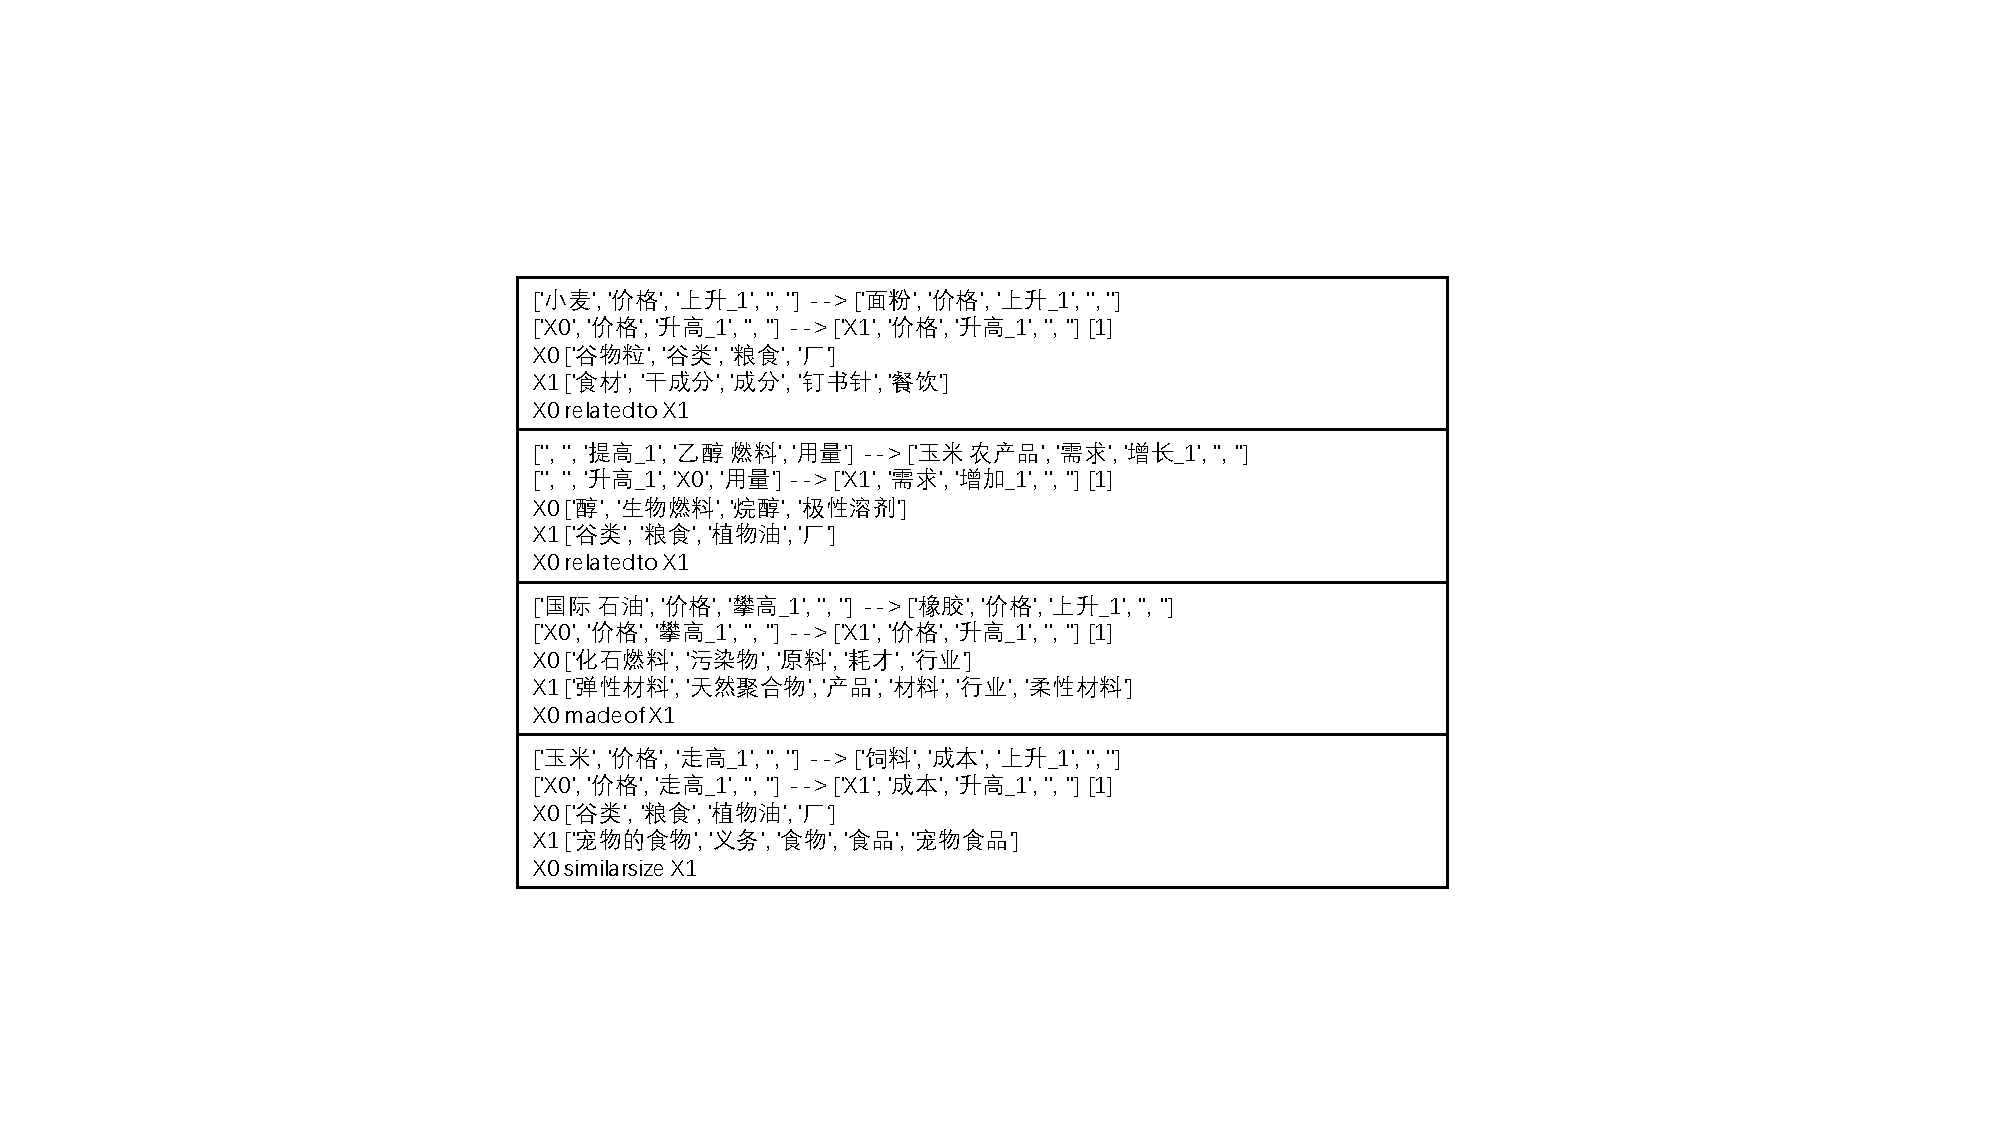
\includegraphics[width=0.95\columnwidth]{figures/reasonable_rule_case}
%	\end{center}
%	\caption{Examples of reasonable Rules.}
%	\label{fig:reasonable_rule_case}
%	\end{figure}
\begin{figure}[htbp]
	\centering
	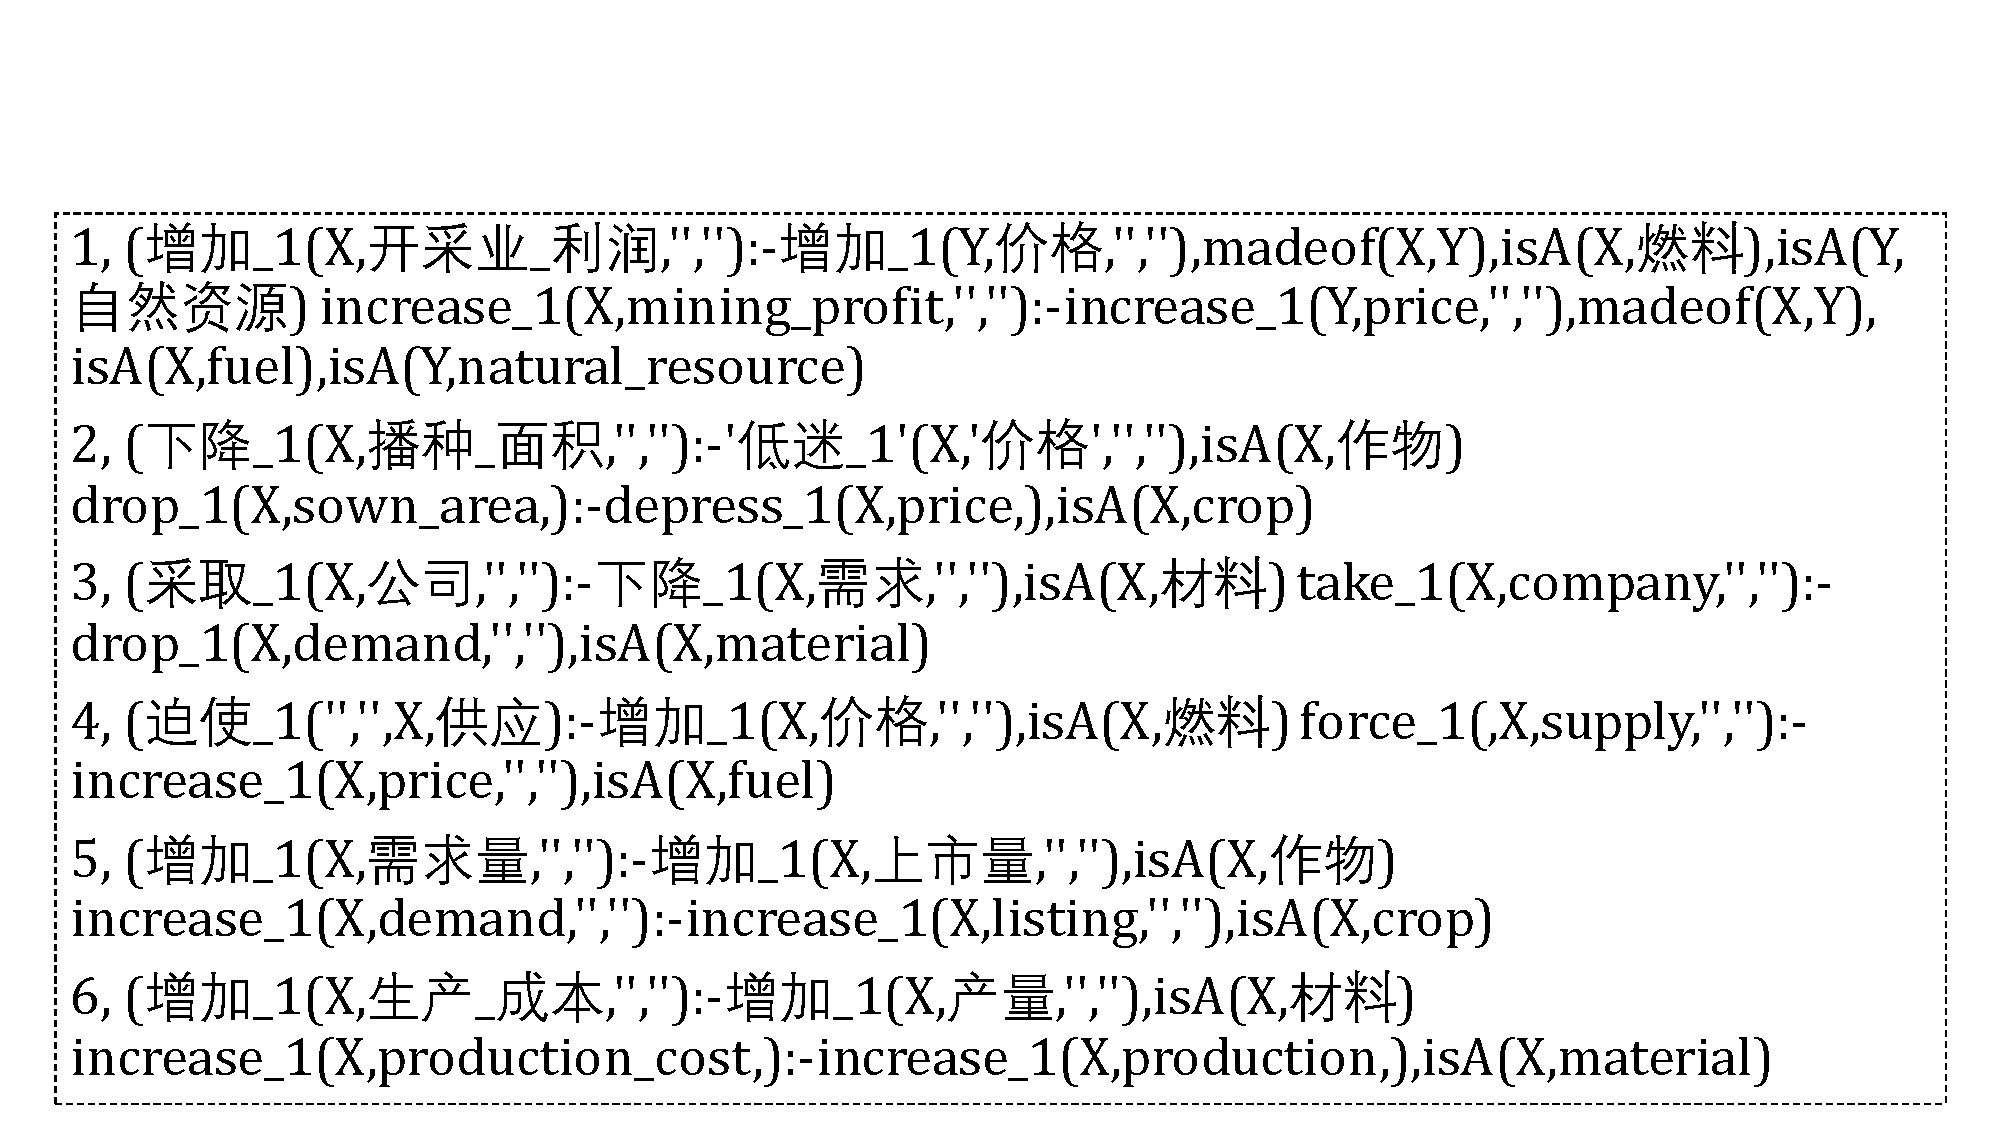
\includegraphics[width=0.95\columnwidth]{figures/rules_case}
	\caption{Examples of Typical Rules}
	\label{fig:rules_case}
\end{figure}
\paragraph{Event Graph}
With these rules, we deduce many rule instances with Prolog and pick out a tiny subgraph about rise and fall events, in Figure\ref{fig:rule_instantiation_graph}, to show the power of the rules. 
	
\begin{figure}[htbp]
\begin{center}
	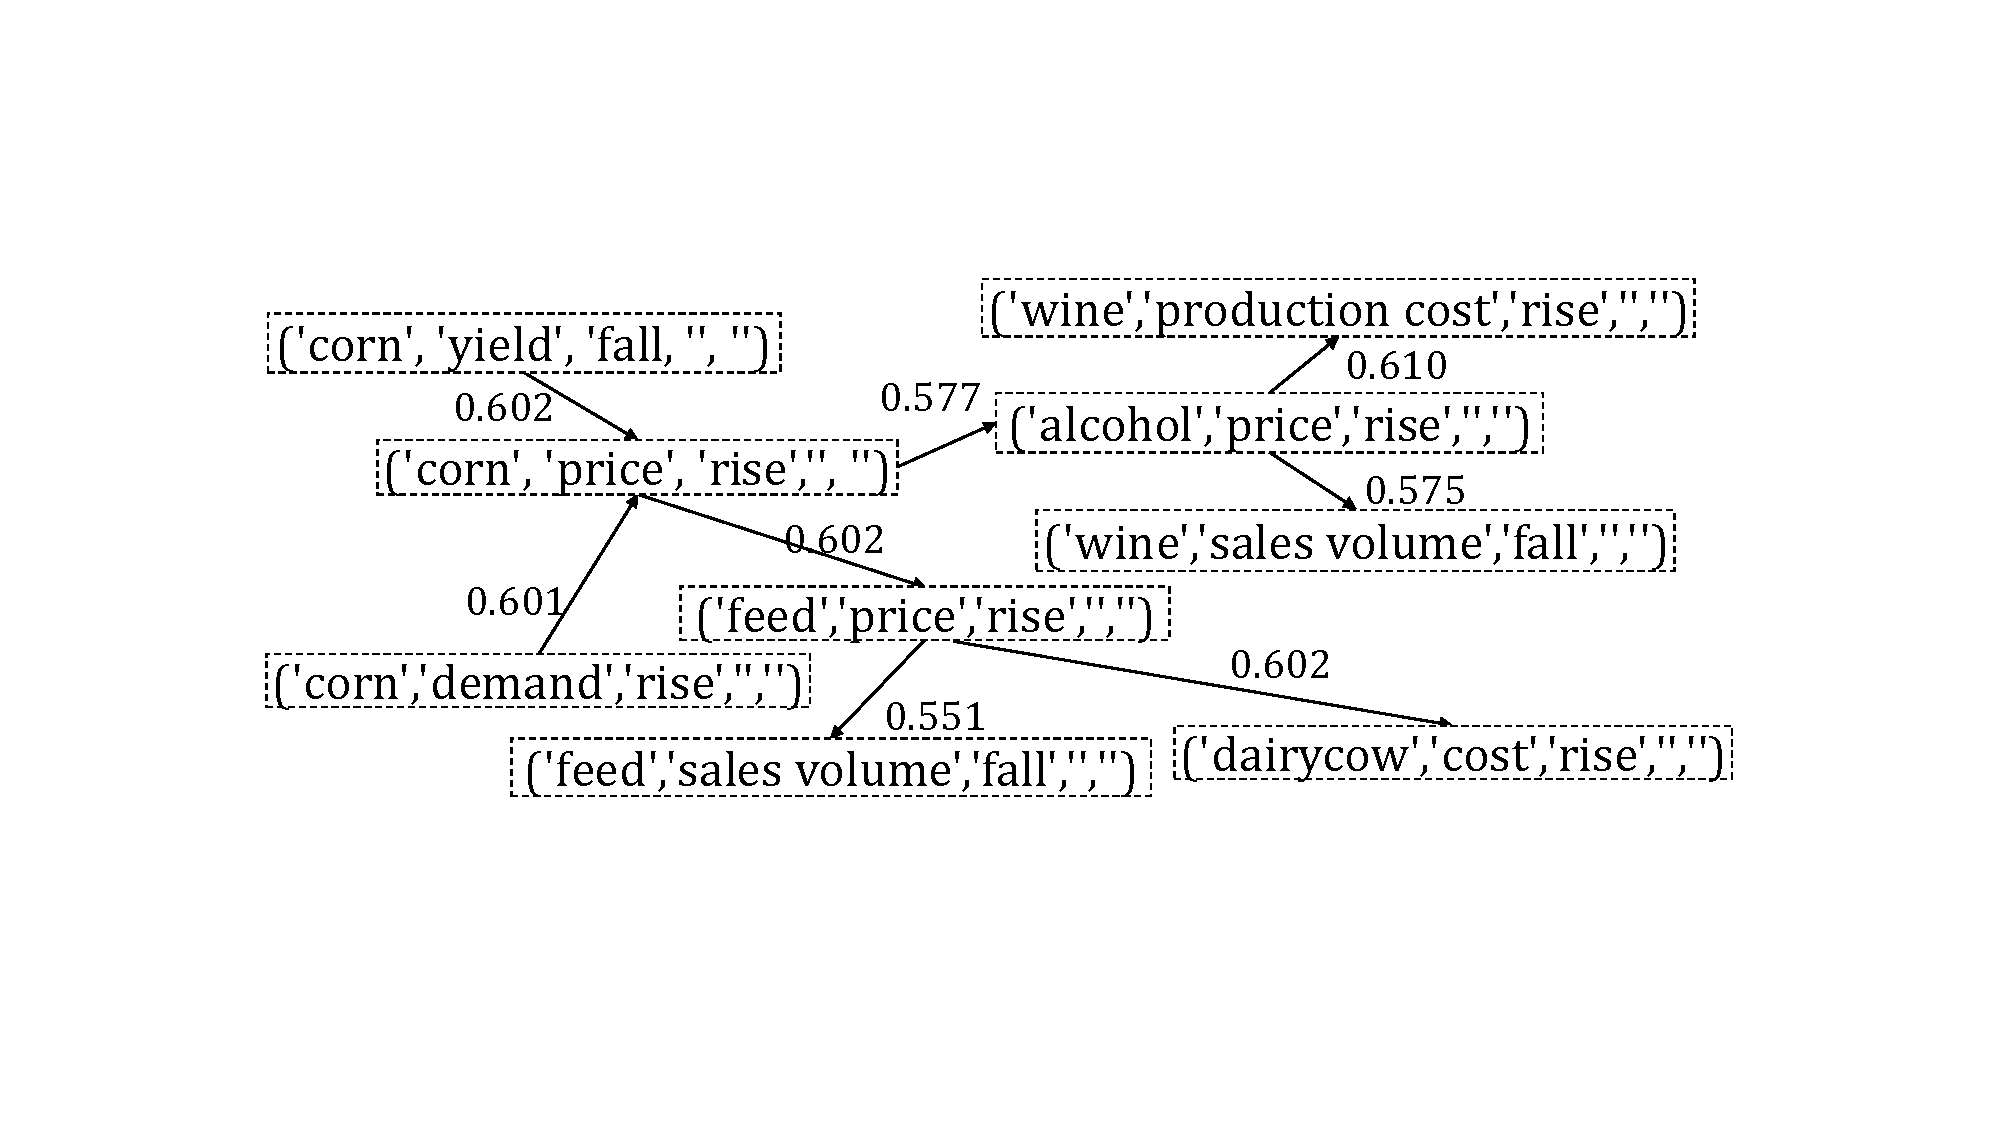
\includegraphics[width=0.9\columnwidth]{figures/instantiation_graph}
\end{center}
\caption{Rule Deduction. As space is limited, we only show the English version and omit the rules used in the reasoning process.}
\label{fig:rule_instantiation_graph}
\end{figure}

\subsection{Comparison with existing Knowledge Bases}
We compare our rules with causal part of other knowledge bases in various aspects in Table \ref{tab:comparison_rule_with_kbs}. We can see our causal knowledge representation is more expressive and informative, and the automatic knowledge acquisition is very convenient.
\begin{table*}[htbp]
\centering
%\begin{tabularx}{\columnwidth}{|c|c|c|c|}\hline
	\begin{tabular}{|c|c|c|c|c|c|c|c|}\hline
	\textbf{Name}&\textbf{Number}&\textbf{Domain}&\textbf{Unit}&\textbf{Data Structure}&\textbf{Information}&\textbf{Source}&\textbf{Precision}\\ \hline
	CausalNet&\textbf{62,675,002}&\textbf{Open}&word&(-)&rich&\textbf{automatic}&-\\
	\multicolumn{8}{|c|}{(`drink',`accident',36)}\\\hline
	ConceptNet &89,416&\textbf{Open}&short text&unstructured&rich&crowdsourcing&\textbf{100\%}\\
	\multicolumn{8}{|c|}{(`smoking',`/r/Causes',`cancer')}\\\hline
	FrameNet&59&\textbf{Open}&frame&\textbf{structured}&richer&crowdsourcing&\textbf{100\%}\\
	\multicolumn{8}{|c|}{Killing(Killer,Place,Means,Victim,Instrument),CausativeOf,Death(Protagonist,Place,Manner,Time)}\\\hline
	ATOMIC&568,312&\textbf{Open}&\textbf{logic event}&semi-structured&much richer&crowdsourcing&86.2\%\\
	\multicolumn{8}{|c|}{If ``PersonX pays PersonY a compliment", Then ``PersonY will smile"}\\\hline
	Ours&50,000&Finance&\textbf{logic event}&\textbf{structured}&\textbf{richest}&\textbf{automatic}&32.5\%\\ 
%			Deductive Rule Instance&\TD{??}\\ 
%	\multicolumn{8}{|c|}{See above rule example in Figure\ref{fig:rules_case}}\\\hline
\multicolumn{8}{|c|}{(Z,`price',`rise',`',`'):-(`',X,`suffer',Y,`attack'),isA(X,`country'),isA(Y,`disaster'),isA(Z,`metal'),atLocation(Z,X) conf:0.842}\\\hline	
	\end{tabular}
%\end{tabularx}  \cite{sap2018atomic}
\caption{Comparison with existing knowledge bases}
\label{tab:comparison_rule_with_kbs}
\end{table*}



%\begin{table}[htbp]
%	\caption{Rule Instance \& Rule}
%	\begin{center}
%	\begin{tabular}{|r|l|}\hline
%		\multicolumn{1}{|c|}{Name}                  & \multicolumn{1}{c|}{Number} \\\hline
%		\multicolumn{1}{|c|}{Rule Instances}        & \multicolumn{1}{c|}{7835403} \\ \hline
%		\multicolumn{1}{|c|}{Rules}                 & \multicolumn{1}{c|}{69036}  \\ \hline
%		\multicolumn{1}{|c|}{more than on relation} & \multicolumn{1}{c|}{2499(3.6\%)}\\
%		\multicolumn{1}{|c|}{only one relation}     & \multicolumn{1}{c|}{66539(96.4\%)} \\
%		\hline
%		==                                          & 56449(84.8\%)                      \\
%		madeof                                      & 5659(8.5\%)                        \\
%		atlocation                                  & 1835(2.76\%)                       \\
%		partof                                      & 1061(1.59\%)                       \\
%		usedfor                                     & 954(1.43\%)                        \\
%		hasa                                        & 511(0.768\%)                       \\
%		derivedfrom                                 & 38(0.0571\%)                       \\
%		hasproperty                                 & 20(0.0301\%)                       \\
%		createdby                                   & 12(0.018\%)                        \\ \hline
%	\end{tabular}
%	\label{tab:rule_statistics}
%\end{center}
%\end{table}
	%Rule Instances & 1817014(4337755)\\
	%Candidate Rules & 86218(201359)\\
	%Rule & 18348(42246)\\

\subsection{Ablation Study}
In this section, we explore the contributions of the various components of our rule learning framework.
\paragraph{Causal patterns statistic} The matched sentences distribution over 3 groups of patterns is shown in Table \ref{tab:pattern_statistics}. All patterns in one group have different causal cue words literally but the same meaning. It shows the third pattern group is more rigorous than the first two groups but has lower usage. Probably because more logical thinking is needed when editing news using more rigorous patterns.

%		\begin{table}[htbp]
%		\caption{Causal patterns. A is a cause tokens span, and B is an effect tokens span. Word '因为' represents a group works like '由于,'是因为','因为','缘于','归因于','原因是','起因','鉴于', and word '所以' represents a group of words like '所以','因而','因此','故此','故而','因故','导致','招致','以致','引致','诱致','致使','造成','使得','从而','从而使','于是','为此'}
%		\begin{center}
%			\begin{tabular}{|c|c|} \hline
%				\textbf{Pattern}& \textbf{Priority}\\ \hline
%				因为 A, 所以B&1\\ \hline
%				A,所以 B&2\\ \hline
%				因为 A,B&3\\ \hline
%			\end{tabular}
%			\label{tab:causal_pattern}
%		\end{center}
%	\end{table}	
	
\begin{table}[htbp]
	\centering
	\begin{tabular}{|c|c|c|c|} \hline
		\textbf{Pattern template}& \textbf{Priority}&\textbf{Number}& \textbf{Rate}\\	\hline 
		因为 A,B&1&2000242&48.32\% \\ \hline 
		A,所以 B&2&1530311&36.96\% \\ \hline 
		因为 A, 所以B&3&576851&14.72\% \\	\hline
	\end{tabular}
	\caption{Number of sentences extracted by causal patterns. A is a cause span and B is an effect span. Word `因为' represents a group works like 由于,是因为,因为,缘于,归因于,原因是,鉴于, and word `所以' represents a group of words like 所以,因而,因此,故而,因故,导致,招致,以致,引致,诱致,致使,造成,使得,从而使,于是,为此}
	\label{tab:pattern_statistics}
\end{table}	
\paragraph{External Knowledge Bases}
The following is some statistics of external knowledge bases used in the rule learning framework. The size of the lexicon is 12,624, obtained from `Industrial classification for national economic activities'\footnote{\url{ http://www.stats.gov.cn/Tjsj/tjbz/hyflbz/}}, which determines which event role in the rule instance can be generalized. 
To our knowledge, most existing Chinese taxonomic knowledge bases, such as CN-Probase\cite{Xu2017}, zhishi.me\cite{Niu2011}, are constructed from online-encyclopedia, which suffer that the concepts inside are far less than Probase and they have no probabilistic character. So we translate Probase to get 11,292,493 Chinese `IsA' pairs.
To our knowledge, there exists no large-scale Chinese commonsense knowledge base, so we translate the English part of ConceptNet and merge the Chinese part to get 2,085,681 Chinese triples.
We randomly sample 500 items from translated Probase and ConceptNet, respectively, and the accuracies after the human evaluation are \textbf{87.8\%}(close to the accuracy of original Probase 92.6\%) and \textbf{91.6\%}.

%\begin{table}[htbp]
%	\centering
%	\begin{tabular}{|c|c|}\hline
%		\textbf{Name}&\textbf{Number}\\ \hline
%		Lexicon&12624\\ \hline
%		Translated Probase &11,292,493(87.8\%)\\ \hline
%		Translated ConceptNet&2,085,681(91.6\%)\\ \hline
%	\end{tabular}
%	\caption{External Knowledge Bases}
%	\label{tab:knowledge_base_statistics}
%\end{table}

%After translation, the number of Chinese IsA pairs is 11,292,493. The number of Chinese commonsense triples is 2,085,681. We both randomly sample 500 items from them, and the accuracy after human evaluation are 0.878 and 0.916 respectively.
%The accuracy of original Probase is 0.926. 
%The number of total Chinese IsA pairs are 11,292,493 which contain concept-instance pairs and concept-subconcept pairs, the. The number of Chinese concepts is 81082 concluding concepts and subconcepts. The number of instances is 158693. The number of Chinese commonsense pairs is 7316977.
%\subsection{External Factual Knowledge Bases}

%From above rule instance extraction submodule, we scan get a rule instances repository. With such huge specific rule instances, we hope to further discover the powerful knowledge hidden in these rule instances. 

%so we generalize such a large amount of rule instances with a more general form. As discussed in Section \ref{sec:intro}, we need to build such a knowledge base. Taxonomy and common sense are two major kinds of knowledge in such knowledge base.
%In our framework, we need to rely on the external Chinese knowledge bases, Chinese Probase and Chinese Conceptnet, to generalize rule instances and add constraints. Most existing Chinese taxonomy knowledge is constructed from online-encyclopedia, such as CN-Probase\cite{Xu2017}. They usually focus more on named entity such as famous movie stars, singer stars, while we care more about the concrete things existed in life such as corn, steel, alcohol and so on.  In addition, they have no probabilistic character. Translation is an effective and efficient approach, we choose to translate Probase, which is a probabilistic taxonomic knowledge base.
%To our knowledge, there exists no large-scale Chinese commonsense knowledge base, so we translate the English part of ConceptNet5 into Chinese and combine the Chinese part.

%	 which is special for this, But it is only for English. We have investigated the CN-Probase\cite{xu2017cn}, but It even can't find the concept of common entities like '中国/China', '橡胶/rubber' and it also limits the usage frequency. So we collect the items from Probase, the items with 'IsA' relation in ConceptNet5\cite{speer2013conceptnet}, Webbrain\cite{chen2016webbrain}. Then, we fuse them together, Then, translate them into Chinese with google translator. to reduce the translate error, we put more context into the translator as more as possible, for example we put 'fruit such as apple, banana', Then we can get the translated result of IsA(apple,fruit), IsA(banana, fruit) together, which can make word sense of 'apple' to be translated near the fruit not company.  
%	\subsubsection{Chinese Commonsense knowledge base.}
%	, consisting of 47, 3, 25 relations respectively. Some of them are duplicative and some are useless for us. So we select specific number useful relations and we also design some patterns to extract some relations from Chinese wiki. 
%	relattions between arguments are used in rule specialization submodule to make rules reasonable. There exist many commonsense knowledge bases such as ConceptNet5, WebBrain, WebChild.  The numbers of the relations in these knowledge bases are limited. And some relations are equivalent among different knowledge bases, such as '/r/RelateTo' in ConceptNet is equivalent to 'relateto' in WebBrain. So we normalize all the relations names literally.
% Meanwhile, many pairs of arguments have more than one relations which are  duplicated semantically. For example, (sweet corn, corn) has the relations 'relatedto' and 'partof', obviously, 'partof' consists of 'relatedto' semantically. So we hope to remove the semantic reduplication relations. which means we need find the semantic containment relations among these relations.
%Algorithm \ref{alg:alg1} shows the Relations Containment algorithm we proposed. It firstly counts each relation and its corresponding arguments pairs. Then, compare the every two correlated relations, and record their containment relation. Last, enumerate all relations in each pair of arguments, remove the relation which is not contained in other relations existed in this pair of arguments.
%When fusing these knowledge bases, we regard arguments from different knowledge bases which have the same literal name as the same arguments.
%	from structured information to knowledge which is close to intelligence
%The goal of rule acquisition is to learn first-order logic rule from huge number of rule instances with the support of external factual knowledge, shown in the Figure \ref{fig:overview}'s middle part.
%with the knowledge base, now, we can generalize the rule instances extracted from rule instances extraction submodule into candidate rules to represent more general knowledge. For example, we hopefully generalize from each cluster of rule instances to one candidate rule. For example, given two rule instances in one cluster, ('国际 石油', '价格', '攀高@攀高', '', '') $->$ ('橡胶', '价格', '上升@升高', '', '') and ('国际 柴油', '价格', '攀高@攀高', '', '') $->$ ('橡胶', '价格', '上升@升高', '', ''), the generalized candidate rule would be('X0', '价格', '攀高', '', '') $->$ ('X1', '价格', '升高', '', '') where 'X0' IsA' 化石燃料','原料' and  'X1' IsA '弹性材料' '天然聚合物'.


%\begin{table}[htbp]
%\centering
%		\begin{tabular}{|c|c|}\hline
%			\textbf{Name}&\textbf{Number}\\ \hline
%			Lexicon&12624\\ \hline
%			Concepts &18281\\	
%			IsA pairs &123547\\
%			Concept-subconcept pairs&18753\\
%			Concept-instance pairs&104794\\\hline
%			Commonsense Pairs&32593\\ 
%			Commonsense Relations&10\\ \hline
%		\end{tabular}
%		\caption{Knowledge Base}
%		\label{tab:knowledge_base_statistics}
%\end{table}
\paragraph{Open Event Extraction}
%	TextRunner/WOE,ReVerb,Ollie,ClausIE,SRL/AMR parsing/frame-semantic parsing,NestIE 
Since our event structure scheme is plain and straightforward, we choose the reliable Stanford CoreNLP tool to extract the rule instances.
%	rule instance  97/200(48.5\%)& 21/200(10.5\%) & 82/200(41.0\%) \\ \hline
The number of rule instances extracted after rule instance distilling submodule is 7,835,403. Since most of them are discarded in the learning process, the number of rule instances really used for rule induction is 78,098 with an accuracy of \textbf{48.5\%} (we also sample 200 rule instances and manually evaluate them).

%\textit{To sum up}, our framework is a pipeline, in which rule instance extraction achieve 48.5\%, ConceptNet5 translation achieve 91.6\% and Probase translation achieves 87.8\%, So teh rule finally can achieve 39.0\%(48.5\%*91.6\%*87.8\%) maximumly, which is close to the evaluation of the final rules. 

%\textbf{\textit{To sum up}}, 
%our framework is a pipeline, in which the accuracy of rule instance extraction is 48.5\%, the accuracy of ConceptNet5 translation is 91.6\%, and the accuracy of Probase translation is 87.8\%. 
\textbf{\textit{To sum up}}, our framework is a pipeline undergoing rule instance extraction(accuracy 48.5\%), constrain relations addition(accuracy of ConceptNet 91.6\%), and rule induction(accuracy of Probase 87.8\%).
Thus, the accuracy can only reach \textbf{39.0\%} (48.5\%*91.6\%*87.8\%) at the maximum, which is close to our evaluation(32.5\%) of the final rules.

%	\subsubsection{Rule Acquisition}
%	\begin{table}[]
%		\centering
%		\begin{tabular}{lll}
%			& rule number  & qualitity       \\
%			no Coneptnet / only one relation    & 66539/96.4\% & informative     \\
%			Conceptnet / more than one relation & 2499/3.6\%   & more infrmative
%		\end{tabular}
%		\caption{Relation Number}
%	\end{table}

%	\begin{table}[]
%		\caption{Event Connection}
%		\begin{center}
%		\begin{tabular}{lll}
%			==         & 60475 & 84.4\%  \\
%			madeof     & 6161  & 8.6\%   \\
%			atlocation & 2104  & 2.94\%  \\
%			partof     & 1152  & 1.61\%  \\
%			usedfor    & 1072  & 1.5\%   \\
%			others     & 674   & 0.941\%
%		\end{tabular}
%		\end{center}
%	\end{table}
\subsection{Application: Futures Price Prediction}
%\paragraph{Reasoning with Uncertainty}
\begin{figure}[htbp]
	\begin{center}
		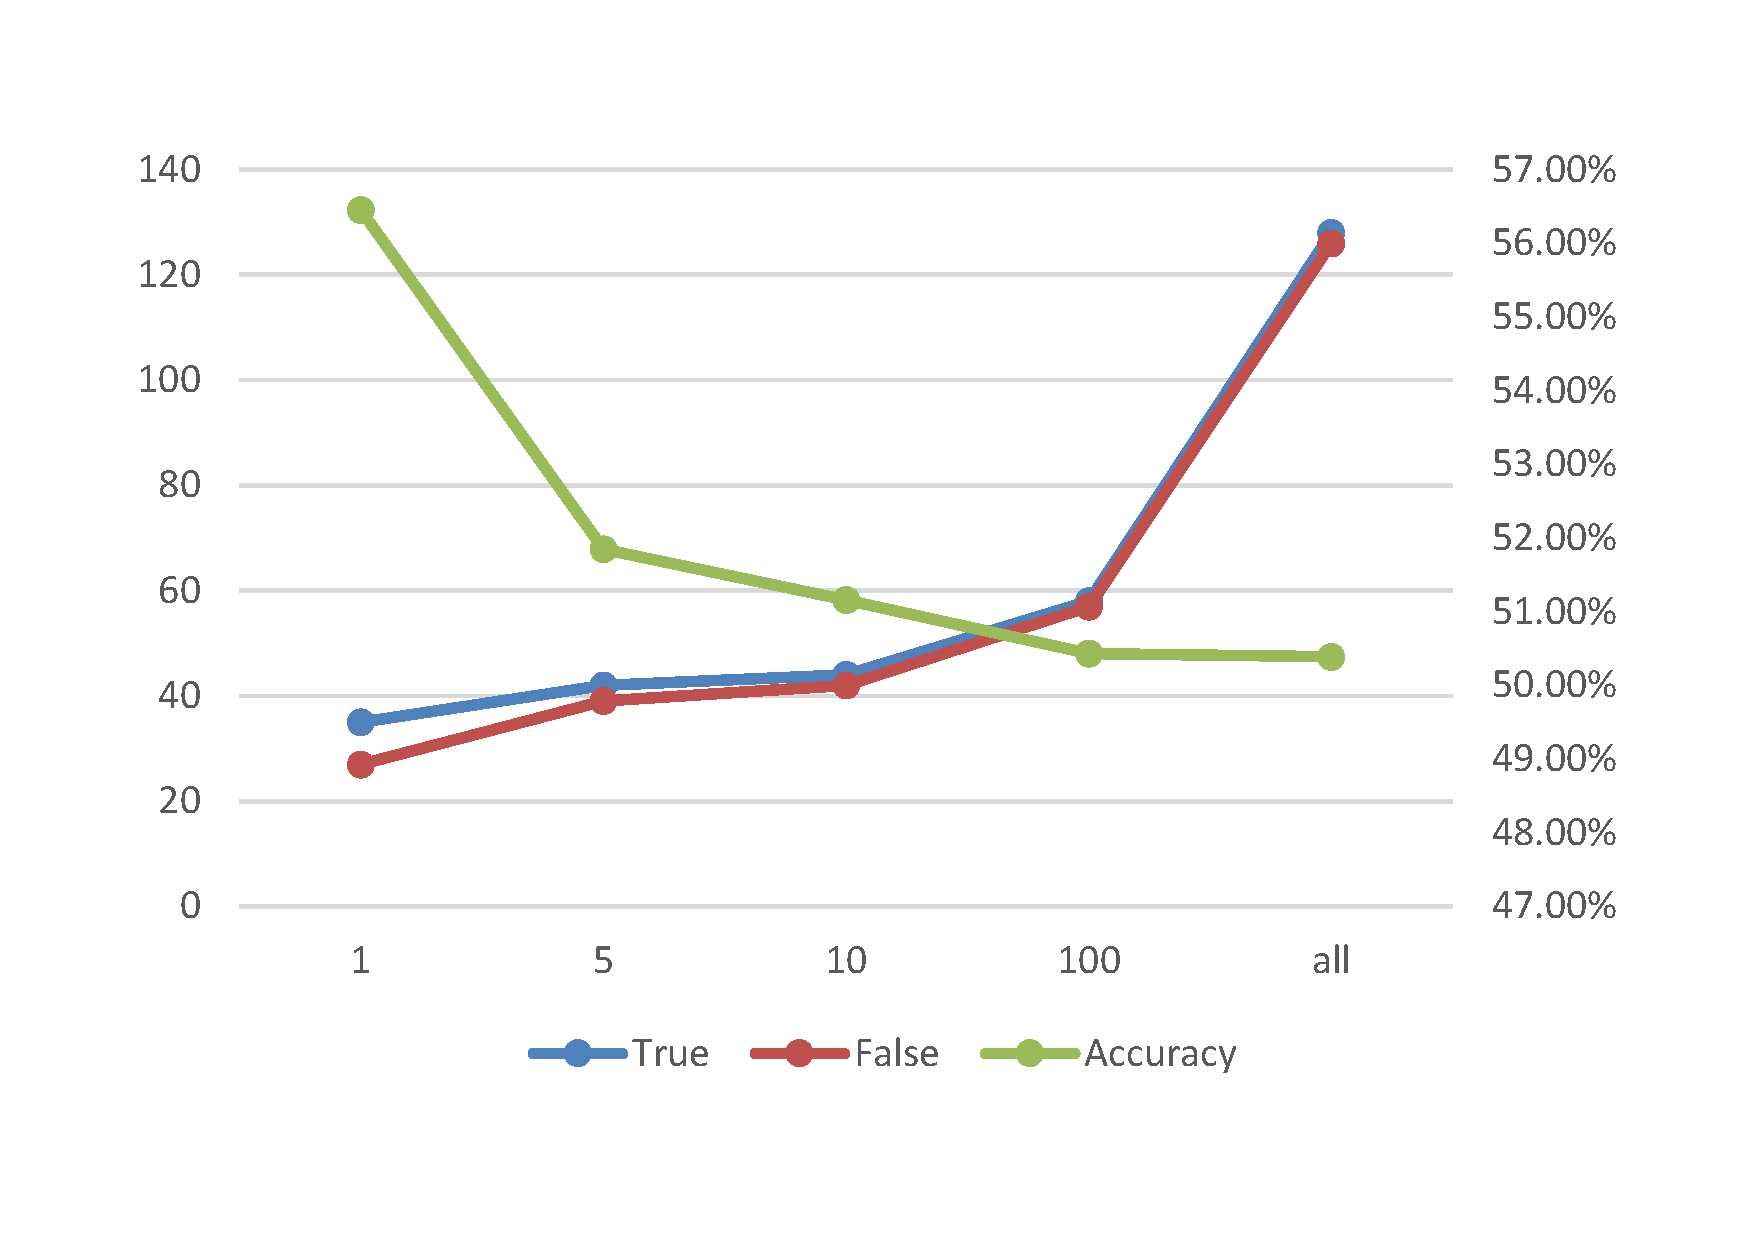
\includegraphics[width=0.9\columnwidth]{figures/rule_futures_prediction}
	\end{center}
	\caption{Futures Price Prediction.}
	\label{fig:futures_price_prediction}
\end{figure}
We choose futures price prediction because the futures are common and concrete things existed in ConceptNet and Probase, such as corn, oil, etc.
%\cite{Ding} is the state-of-the-art stock prediction model(EB\_CNN). We follow similar experimental settings. 
We follow similar experimental settings in \cite{Ding}.
From 2018/1/1 to 2018/11/2, we collect all the headlines and the price change of 15 futures as test data, which include \textbf{851} price change events (The price change of more than 1\% relative to the previous day is an event and we only focus on rise or fall events). 

Baseline models: EB\_CNN model \cite{Ding}, the state of the art model in stock price prediction, uses a deep convolutional neural network to model both short-term and long-term influences of events on stock price movements, and the accuracy of futures prediction is \textbf{54.2\%}. Other models in \cite{Ding}, such as EB\_NN, WB\_CNN, and WB\_NN can achieve \textbf{53.0\%}, \textbf{53.2\%}, and \textbf{53.5\%}, respectively. These accuracies of futures prediction are lower than the accuracies of stock prediction shown in the paper.
It may be because the factors affecting the futures price are far less than the stock price and the futures price is much more stable than the stock price, which makes useful training information about the futures less and further affects the accuracy of the models.

Our approach: For each actual future price change event , we get the news headlines for the previous month before this event. 
For each news headline, we extract the event, use Prolog to reason based on the rules and external knowledge bases, and get the top K inferred events sorted by the confidence.
We may have m*K inferred events for this event, m is the number of events occurred in this month. 
Here, we select the price change events(rise or fall) of the future in this actual future price change event from m*K events and calculate the weighted sum of their confidences(rise event weights 1 and fall event weights -1). If the sum value is positive, we predict this future price as a rise event, otherwise as a fall event. If get no related events changing the future's price, do not make prediction. We compare this prediction with the actual price change to evaluate the reasoning effect. 
Figure \ref{fig:futures_price_prediction} shows the average prediction result. It shows the more predicted events inferred from the Prolog(by increasing K) we use, the lower the prediction accuracy is(from \textbf{56.5\%} to \textbf{50.4\%}), and the more futures events we can predict(from \textbf{62} to \textbf{254}). 

\textbf{\textit{To sum up}}, our rule-based prediction approach can have a higher prediction accuracy (56.45\%) and better interpretation ability with a low recall rate, which is very practical in life.

%\begin{table}[htbp]
%	\caption{Baselines and Proposed Framework}
%	\begin{center}
%		\begin{tabular}{lll}\hline
%			& Acc & MCC \\\hline
%			WB-NN &  0.535 &     \\
%			WB-CNN&  0.532  &     \\
%			EB-NN &  0.530  &     \\
%			EB-CNN&  0.542   &     \\
%			Rule &     &    \\\hline
%		\end{tabular}
%		\label{tab:baselines_and_rule}
%	\end{center}
%\end{table}

\subsection{Downloading and Demo}
The translated Chinese Probase and ConceptNet and learned rules are available at URL.
We built a demo to demonstrate the reasoning process at URL. 
We also developed an application demo of futures prices change triggering that can monitor news from around the world in real time, find the news that may cause futures prices changes, and alert users. Visit URL.
\section{Related Work}
\paragraph{Clarification Question Generation} The concept of CQ can be naturally raised in a dialogue system where the speech recognition results tend to be erroneous so that we raise CQs for sanity check \citep{stoyanchev2014towards}, or the intents for a task is incomplete or ambiguous in a first short utterance and further CQs are needed to fill in the slots \citep{dhole2020resolving}. The concept is then extended to IR to clarify ambiguous queries \citep{aliannejadi2019asking}, and has been successfully put into practice \citep{zamani2020generating}. Other application areas including KBQA \citep{xu2019asking} and open-domain dialogue systems \citep{aliannejadi2020convai3}. CQGen can also be applied to help refine posts on websites like StackExchange \citep{Kumar_2020} and Amazon \citep{rao2019answer}. In this context, our work closely follows the research line of \citep{rao2018learning, rao2019answer, cao2019controlling}. \citet{rao2018learning} first adopted a retrieval-then-rank approach. They \citep{rao2019answer} then proposed a generation approach to train the model to maximize the utility of the hypothetical answer for the questions with GAN, to better promote specificity. \citet{cao2019controlling} propose to control the specificity by training on data with explicit indicator of specificity, but it requires additional specificity annotation. Towards the similar specificity goal, we adopted a different keyword-based approach. They also assume generating one question per context, which we claim is not sufficient to cover various possible information needs, and thus propose the task of the diverse CQGen.

\paragraph{Diverse Generation} The demand for diverse generation exists in many other fields~\cite{vijayakumar2018diverse, LiangZ18code, shen2019mixture}, and we've drawn inspirations from these literatures. For image captioning, we may use multiple descriptions for different focusing points of a scene. \textit{Diverse Beam Search} \citep{vijayakumar2018diverse} was proposed to broaden the searching space to catch such diversity by dividing groups in decoding and imposing repetition penalty between them. For machine translation, a context can be translated with different styles. \citet{shen2019mixture} thus proposed \textit{Mixture of Expert} models including hMup to reflect various styles with a discrete latent variable (\textit{expert}). And here for CQGen, diversity is required to cover various potentially missing aspects, so we come up with the idea to use keywords as a controlling variable like \textit{expert} to promote diversity.


\section{Conclusion}

In this paper, we incorporated the idea of Cookie Theft picture description task into the evaluation of the high-level cognitive abilities of LVLMs and designed a novel evaluation benchmark called CogBench.
% Images in CogBench are of high quality and require more cognitive reasonings to understand, which makes it different from existing image datasets.
The images in CogBench are of high quality and demand more complex cognitive reasoning for interpretation, setting it apart from existing image datasets.
% It consists of a image description task and a VQA task.
Experiments show that there is still a large gap between the cognitive abilities of LVLMs and human beings, indicating CogBench is a challenging benchmark.

% In the future


\bibliographystyle{ACM-Reference-Format}
\bibliography{ref}

\end{document}
